\documentclass[../PFC.tex]{subfiles}
\begin{document}

\section{Introducción}
\label{App:Introducción}

Anteriormente se han explicado los conocimientos y términos generales relacionados con la seguridad en la autenticidad NFC basada en criptología con curvas elípticas. A continuación se muestra la aplicación de dichos conocimientos en un proyecto software experimental. El objetivo es demostrar la capacidad de los dispositivos NFC para, de la mano de la criptografía con curvas elípticas, llegar a desarrollar un sistema de autenticación eficiente y fiable.
\\\\
Tanto los nombres, librerías, herramientas, así como el resto del material utilizado se describirán a continuación. A su vez, siguiendo un estándar de desarrollo software basado en metodologías ágiles, se mostrará la utilizada para éste proyecto. Para ello,  el autor y director de este TFG (Fidel Abascal y Domingo Gómez) hemos actuado y ejercido tanto de cliente como de contratado para el desarrollo de la aplicación. 
\\\\
Dentro de un ámbito ficticio, se plantea una empresa llamada \textbf{Alpha - Consultora S.A.}\footnote{Cualquier similitud con la realidad es mera coincidencia}, nueva potencia local dentro del campo de la seguridad bancaria, que ha cosechado unos excelentes resultados a lo largo de sus 2 años de existencia. Cuenta con más de 40 trabajadores y su crecimiento y expansión es notoria. Tanto es el éxito de esta compañía que, para dar cabida a su plantilla, ha decidido trasladarse a una nueva sede más moderna, amplia y mejor ubicada. La empresa, antes de instalarse en la nueva sede, decide contratar a unos expertos en seguridad para gestionar el control de accesos mediante un sistema de tarjetas y lectores en las entradas; teniendo en cuenta una inversión mínima pero garantizando un alto grado de seguridad.
\\\\
Tras buscar incesantemente recurren a la empresa \textbf{F-NFC}. Una vez realizado el estudio por parte de F-NFC, se pone en consonancia un acuerdo para elaborar una aplicación que genere información que autentifique a un usuario de la empresa \textit{Alpha} y sea reconocido de forma unívoca para permitir su acceso a la sede. La infraestructura de la empresa propietaria de la nueva sede corresponde a la figura \ref{img:infraestructura}.

\begin{figure}[!ht]
  \centering
  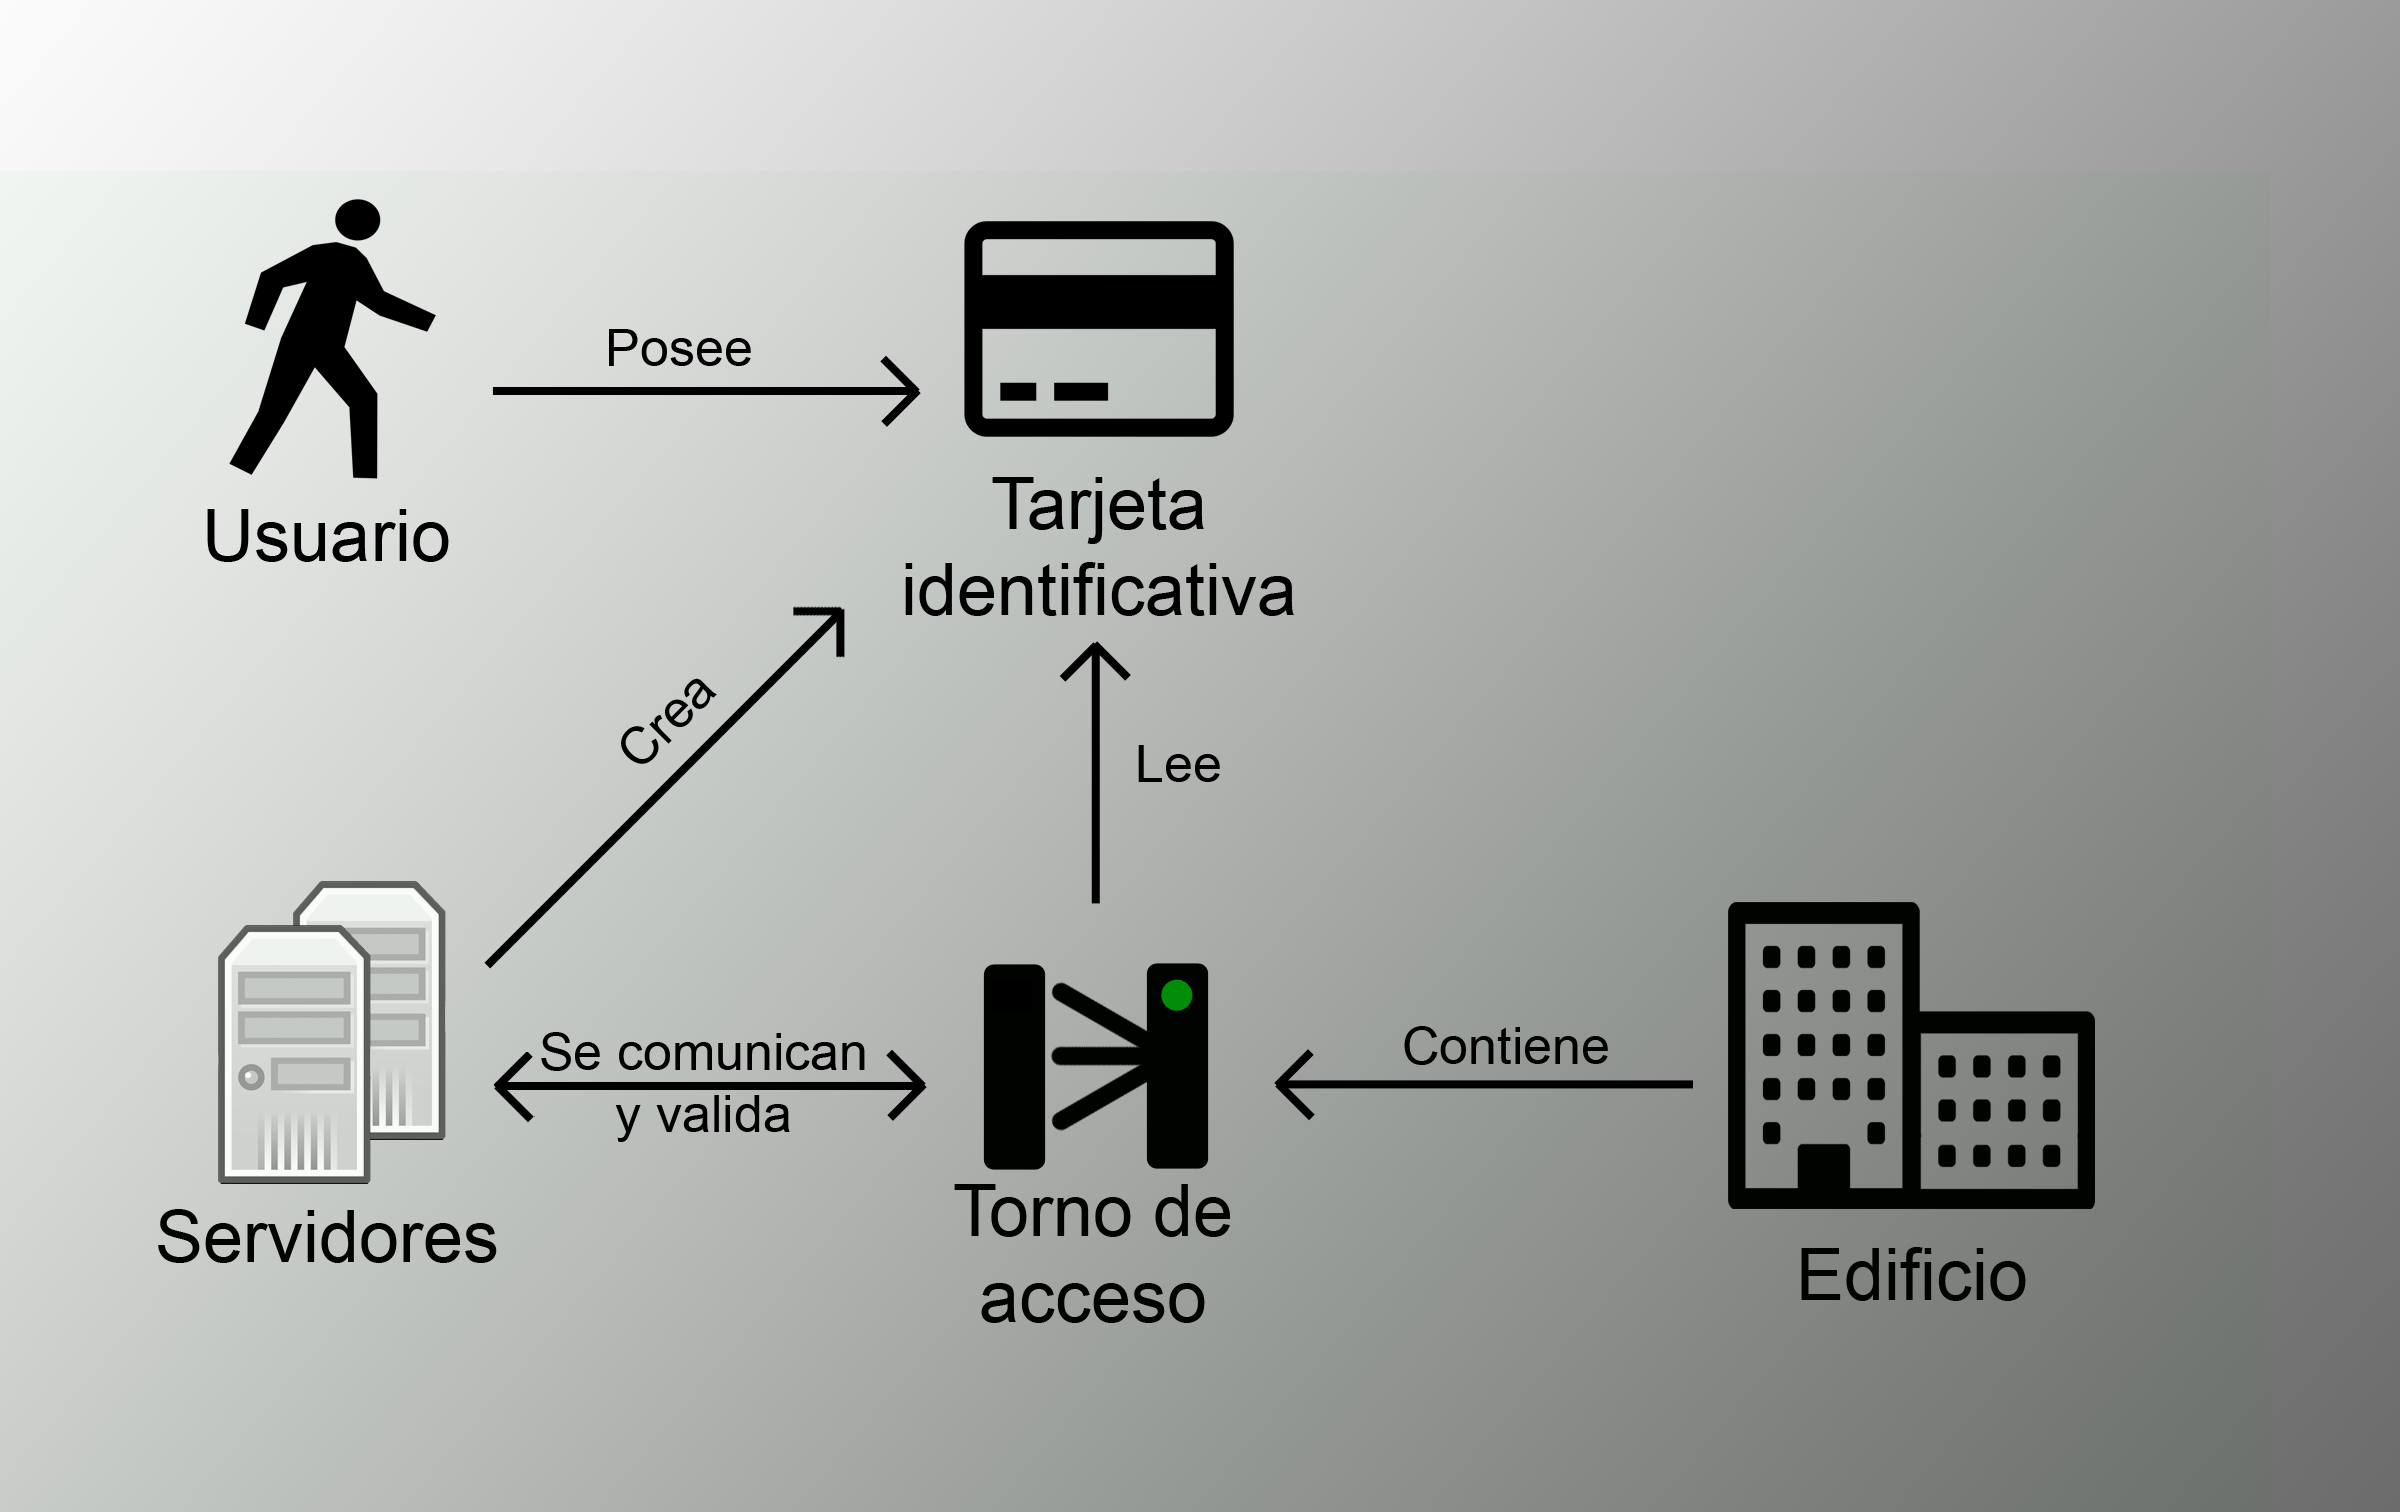
\includegraphics[width=1\textwidth]{./img/arquitecturaVirtual}
  \caption{Infraestructura del sistema ficticio.}
  \label{img:infraestructura}
\end{figure}

Los detalles de implementación de la aplicación seguirán un objetivo didáctico y experimental que cumplirán los requerimientos de la situación propuesta; adecuándose a la carencia real de la infraestructura anteriormente mencionada. Se explicará en las secciones siguientes en detalle todos los puntos implicados en la consecución de este objetivo. Más concretamente en el apartado de escenario de la aplicación \ref{App:Escenario}.

\section{Materiales y tecnologías utilizadas}
\label{App:Materiales y tecnologías utilizadas}

Para el desarrollo del proyecto se ha utilizado, ante todo, software de carácter libre junto a imágenes, textos, estructuras y contenido sin restricciones de uso. Ya sea debido al tipo de licencia de cada elemento o por ser de autoría propia.
\\\\
El desarrollo se ha realizado en el lenguaje de programación \textit{Java} con el kit de desarrollo \textit{Java} (JDK) 1.8.65 (\textit{Java 8 update 65}) de \textit{Oracle Corporation}\cite{java}.
\\\\
El entorno de desarrollo integrado o \textit{IDE} de la aplicación es el oficial de Google para el desarrollo para dispositivos \textit{Android}: \textit{Android Studio}, versión 1.5.1\cite{androidStudio}. Este programa provee las herramientas básicas de desarrollo; entre ellas, un administrador de los kit de desarrollo o \textit{SDKs} para las diferentes versiones y varios elementos descritos a continuación: 
\begin{itemize}
\item{Plataformas SDK}
	\begin{itemize}
	\item{API 22: Para la versión Android 5.1.1.}
	\end{itemize}
\item{Herramientas SDK}
	\begin{itemize}
	\item{Android Build Tools : Para la construcción de la aplicación.}
	\item{Android SDK Platform Tools v23.1: Soporte para el desarrollo.}
	\item{Repositorio de ayuda Android, rev 30.}
	\item{Libreria de ayuda Android, rev 23.2.1 : Ayudas en la retrocompatibilidad 	de elementos de interfaz de usuario.}
	\item{Google USB Driver, rev 11 : Conexión entre el servicio de ejecución de la aplicación y los dispositivos USB.}
	\item{Intel x86 HAXM, rev 6.0.1 : Aceleración \textit{hardware} para la emulación.}
	\end{itemize}
\end{itemize}

Estos componentes de \textit{Android Studio} hacen posible el desarrollo de la aplicación objetivo. Este programa, con carencias notorias en ciertos apartados, ha hecho complicado, de cierta forma, la selección de componentes a instalar, versiones , etcétera debido a diversos motivos de compatibilidades de librerías y actualizaciones desfasadas entre los componentes y el propio IDE. 
\\\\
La esencia de la aplicación reside en la criptografía mediante curvas elípticas. Para la implementación de ello ha sido necesario utilizar una librería externa llamada \textit{Bouncy Castle}\cite{bouncyCastle} versión 1.54. Dicha librería suple las deficiencias de la implementación base de la propia API (\textit{Application Programming Interface}) de \textit{Java} en su paquete de \textit{java.security}\cite{javaSecurity}. La cual tiene limitaciones claras a la hora de la generar curvas elípticas. Gracias a ésta librería se ha podido realizar la parte crítica de la aplicación con una mejora de rendimiento notoria si se tuviera que haber utilizado únicamente la API de \textit{Java}. 
\\\\
Respecto al almacenaje de datos se ha optado por utilizar una pequeña base de datos en \textit{SQLite}\cite{sqlite} descrita más adelante.Ésta base de datos se utiliza para el almacenamiento de unos pequeños registros que utiliza la aplicación. El uso de una base de datos de mayor capacidad y funcionalidades no se ha contemplado factible. 
\\\\
En cuanto a los elementos gráficos de la aplicación, un alto porcentaje son de elaboración propia mediante programas de edición de imágenes. El resto son de libre uso comercial. La iconografía de la aplicación es autoría de \textit{Google Inc.}\cite{googleIcons}. Dichos iconos han de ser vectoriales debido a la optimización del tratamiento de imágenes y su renderizado, por lo que en este aspecto, \textit{Google} provee estos  iconos en formato \textit{SVG} (\textit{Scalable Vector Graphics}) y \textit{PNG}; también \textit{Android Studio} contiene iconografía de forma nativa pero no actualizada. A la hora de incluir estos elementos externos se ha transformado las descripciones vectoriales \textit{SVG} en formato \textit{XML} (\textit{eXtensible Markup Language}) interpretable de forma sencilla por \textit{Android Studio} y fácilmente modificables en los casos que se ha requerido. En el apartado \ref{App:Diseño y aspecto} de diseño y aspecto de la aplicación se comenta en detalle el resto de la disposición, motivación y elaboración gráfica de la aplicación. 
\\\\
La API objetivo del proyecto \textit{Android} ha sido la número 22. Desarrollada para la versión 5.1. (\textit{LOLLIPOP MR1}). Se ha decidido utilizar esta API debido a las mejoras sustanciales en cuanto al trabajo del adaptador NFC implementadas desde la versión 5.0\cite{androidAPI21} y mejoradas en ésta\cite{androidAPI22}. 
\\\\
Para el testado de la aplicación \textit{Android Studio} se dispone de la tecnología \textit{AVD} para la virtualización de dispositivos \textit{Android}. Sin embargo, el rendimiento es pobre en comparación con el testeo y \textit{debug} en un dispositivo físico. Por lo que se ha utilizado un dispositivo \textit{Android} \textit{smartphone} \textit{One Plus One} de la compañía americana \textit{Never Settle}, el cuál dispone de la versión \textit{Android} 5.1.1 y \textit{Cyanogen OS} 12.1.1  en el momento de la elaboración de la aplicación. 

\begin{figure}[H]
  \centering
  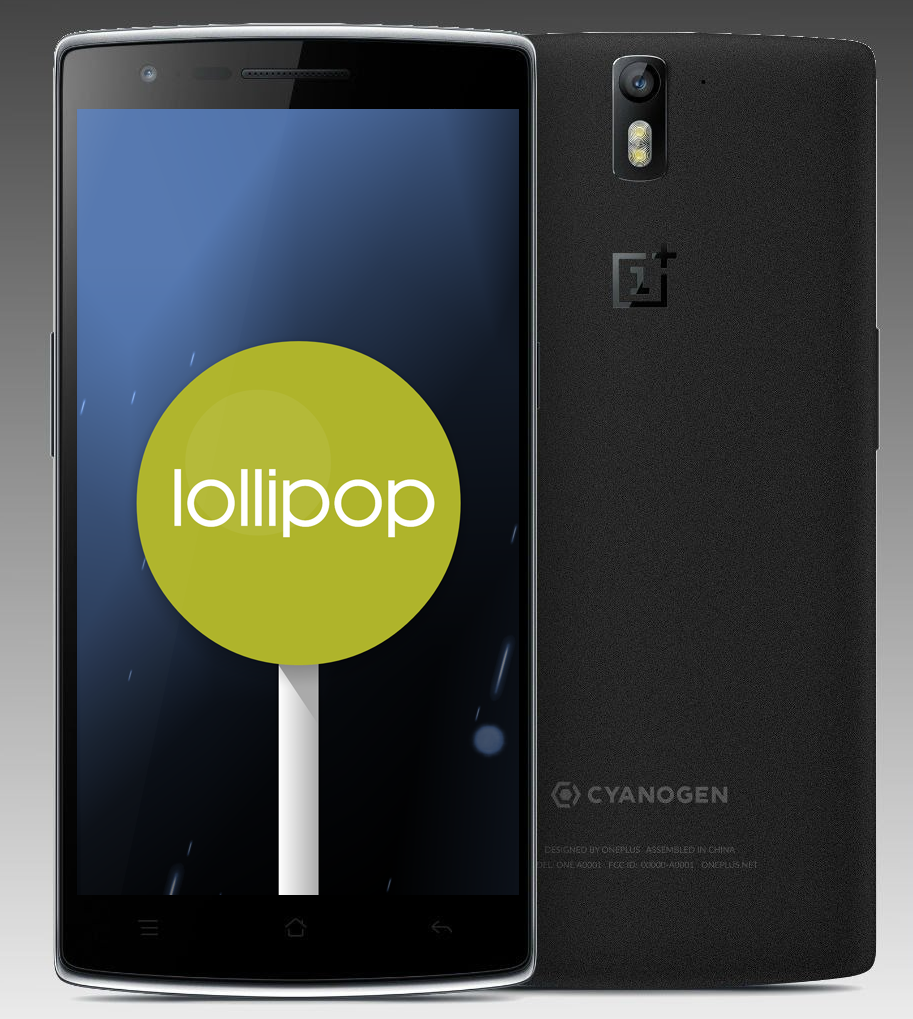
\includegraphics[width=0.4\textwidth]{./img/opo}
  \caption{Smartphone One Plus One - Never Settle}
  \label{img:opo}
\end{figure} 

Por último, el proyecto ha necesitado de dos elementos físicos principales: el dispositivo \textit{Android} mencionado anteriormente y de tarjetas NFC. Debido a la carencia de un presupuesto, se ha optado por utilizar etiquetas adesibles (desde ahora NFC-T) de bajo coste. Se trata del chip \textit{NTAG213} que siguen el estándar ISO 14443-3\cite{iso14443}. Las características de estas etiquetas son las siguientes:

\begin{itemize}
\item{Tipo de etiqueta : ISO 14443-3A.}
\item{Descripción : NXP MIFARE Ultralight (Ultralight C) - NTAG213.}
\item{Tecnología : NfcA, Ndef, MifareUltralight.}
\item{Formato de datos: NFC Forum Type 2.}
\item{Diámetro: 25 mm.}
\item{Identificadores del chip.}
	\begin{itemize}
	\item{Valor ATQA: 0x0044.}
	\item{Valor SAK: 0x00.}
	\item{Firma: NXP Public Key.}
	\end{itemize}
\item{Tamaños y capacidad.}
	\begin{itemize}
	\item{Memoria: 45 páginas de 4bytes por página (180 bytes).}
	\item{Tamaño: 137 bytes.}
	\item{\textit{UID} (Identificador del contenido): 7 bytes\cite{nfcSpecifications}.}
		\begin{itemize}
		\item{\textit{Byte 7}: Valor \textit{UTF-8}, codificación.}
		\item{\textit{Byte 6}: Valor \textit{0}, reservado para uso futuro.}
		\item{\textit{Byte 5-0}: Tamaño del código del lenguaje \textit{IANA}.}
		\end{itemize}	
	\item{Tamaño utilizable: 130 bytes (Tamaño menos \textit{UID}).}	
	\end{itemize}
\end{itemize}

Estas etiquetas se pueden adherir en una superficie que le haga de soporte. Por ejemplo, se podría plastificar junto a dos tapas que cubran el chip y tener la apariencia de una tarjeta común. En la figura \ref{img:nfctag} se muestra una de estas etiquetas. 

\begin{figure}[H]
  \centering
  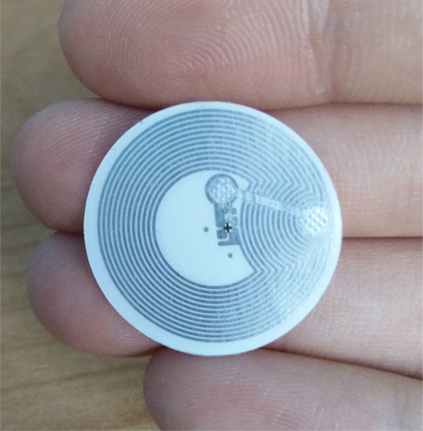
\includegraphics[width=0.5\textwidth]{./img/nfctag}
  \caption{NFC Tag - NTAG213}
  \label{img:nfctag}
\end{figure}

Hubiera sido preferible utilizar chips \textit{MIFARE}\cite{mifare} que tienen mayor capacidad y con mayores funcionalidades como los chips \textit{MIFARE classic} 1K y 4K del productor \textit{NXP}. Estos chips están implementados en una enorme cantidad de aplicaciones en todo el mundo, un ejemplo claro de su uso son en las tarjetas de transporte o hasta en las tarjetas de crédito y la mayoría de chips NFC actuales que impliquen la necesidad de encriptación (RSA comúnmente) y seguridad. En estas tarjetas es realmente complicado acceder a su contenido ya que se precisan ciertas claves para la lectura y decodificación. Sin embargo, en las utilizadas en este proyecto se escribe en texto plano (siguiendo el objetivo didáctico); en el apartado de seguridad y criptología \ref{App:Seguridad y criptología} se explica cómo afectaría esta carencia al sistema final. 
\\\\
Todos los elementos descritos en este apartado conforman lo necesario para simular la estructura descrita en la figura \ref{img:infraestructura} y la implementada definida en el apartado \ref{App:Escenario}. 
\\\\

\section{Metodología}
\label{App:Metodología}

Se ha decidido implementar una metodología de desarrollo software basada en iteracciones de funcionalidades de forma incremental. Para una planificación estructurada se han programado los hitos y la consecución de tareas a completar en cada hito de validación.
\\\\
Gracias a la herramienta Gantt\cite{gantt} para la elaboración de diagramas de planificación de proyectos, se han propuesto gráficamente la duración de cada tarea valorando su dificultad y las posibles modificaciones que hubieran podido surgir de las mismas en cada hito de validación. La duración de cada tarea implica los días necesarios para su finalización; sin tener relación con las horas laborales ya que, aunque no venga reflejado, se ha realizado trabajo en días no laborables. En las figuras \ref{img:gantt-base}, \ref{img:gantt1} y \ref{img:gantt2} se observa la organización inicial planteada. Cada apartado principal de la aplicación precedida de un hito se considera una iteracción incremental del proyecto para adecuarse a la metodología planteada.

\begin{figure}[H]
  \centering
  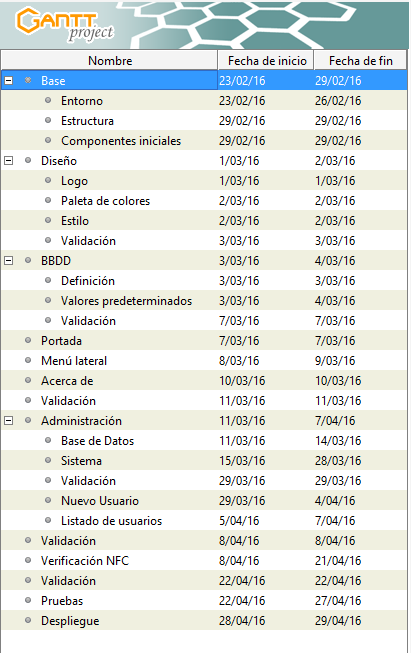
\includegraphics[width=0.4\textwidth]{./img/gantt-base}
  \caption{Diagrama Gantt - Subdivisión de elementos de la aplicación para su desarrollo}
  \label{img:gantt-base}
\end{figure}

\begin{figure}[H]
  \centering
  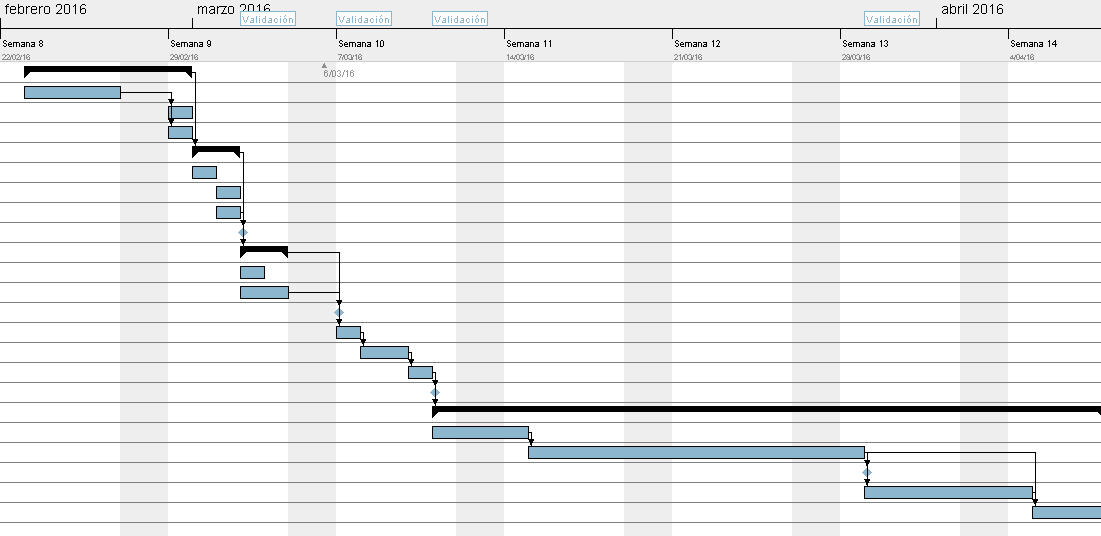
\includegraphics[width=0.8\textwidth]{./img/gantt1}
  \caption{Diagrama Gantt : Visualización (I).}
  \label{img:gantt1}
\end{figure}

\begin{figure}[H]
  \centering
  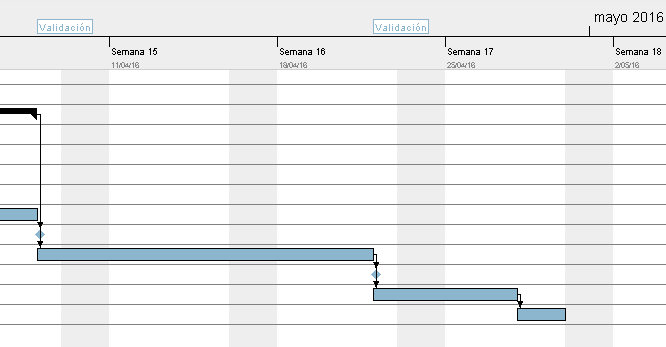
\includegraphics[width=0.8\textwidth]{./img/gantt2}
  \caption{Diagrama Gantt : Visualización (II).}
  \label{img:gantt2}
\end{figure}

Como se puede observar, la duración final del proyecto ha sido de 10 semanas aproximadamente. Con pequeñas variaciones, los hitos se han ido finalizando satisfactoriamente hasta comprobar que todas las tareas y partes del proyecto se han completado correctamente. A esta planificación habría que añadir el tiempo previo necesario para el estudio y preparación para el uso de las herramientas y la tecnología utilizada.

\section{Escenario}
\label{App:Escenario}

La idea principal del escenario de la aplicación se ha comentado en el apartado \ref{App:Introducción}, en donde se comenta que el objetivo de la aplicación es meramente didáctico y experimental. Alejándose de los modelos pragmáticos del desarrollo profesional. 
\\\\
La complejidad añadida de implementar un sistema cercano a la realidad aplicaría un coste elevado de recursos sin tener relevancia notoria en la finalidad comentada; elementos tales como: servidores, \textit{WebServices}, \textit{frameworks} de desarrollo, certificación, optimización, etcétera. Dado que la esencia de este TFG se centra en el elemento teórico y didáctico de la criptología en curvas elípticas, la creación de una aplicación de carácter altamente profesional le añadiría beneficios nimios, los cuales no compensan la complejidad agregada. Por tanto, se han realizado labores de simulación y ciertas partes que se han considerado prescindibles han sido descartadas.
\\\\
La arquitectura de la aplicación representada en la figura \ref{img:infraestructura} muestra un escenario típico que da pie a la implementación de este tipo de seguridad. Dentro de este proyecto virtual se dispone de un edificio el cuál posee tornos o puertas de acceso. Estas puertas son capaces de leer el contenido de las tarjetas NFC de cada usuario del sistema. El contenido de las tarjetas se transmite a los servidores de validación de la empresa (sin la necesidad de que se encuentren físicamente dentro del mismo edificio). Los servidores validarán la información recogida en el torno de acceso y validará o no el contenido. Si resulta validado el torno recogerá de los servidores la nueva información a escribir en la tarjeta para hacer válida el paso la próxima vez. Finalmente, el usuario por medio de ésta tarjeta unipersonal podrá acceder al edificio autenticándose en la entrada.
\\\\
Descrito el escenario virtual, es necesario comentar el escenario real del proyecto se ha realizado. Contando con los elementos del apartado \ref{App:Materiales y tecnologías utilizadas} se agrupan las funcionalidades del escenario virtual en el dispositivo \textit{Android}. Por lo tanto, no hay conexiones a elementos externos y toda la estructura se compone únicamente del dispositivo \textit{Android} y las tarjetas NFC. A su vez, cuenta con las siguientes funciones que simulan las labores del escenario virtual:

\begin{itemize}
\item{Información sobre los usuarios del sistema: En lugar de contar con un acceso a una base de datos que recoja la información, se utiliza una pequeña base de datos dentro del dispositivo que contiene la información básica de los usuarios (identificador y nombre del usuario).}
\item{Información del sistema de encriptación: El dispositivo también contiene la información básica del criptosistema implementado (labor de información de servidores).}
\item{Validación: Tras leer el contenido de la tarjeta NFC, denegará o validará la información obtenida (labor de validación y acceso).}
\item{Funciones de administración del sistema: El dispositivo es capaz de restaurar los valores por defecto del sistema, junto a la información inicial. También permite crear nuevas definiciones del sistema de seguridad. Por último, también asignará usuarios al sistema de seguridad que no se encuentren dentro (labor de creación de tarjetas).}
\end{itemize}

Gracias a esta implementación del escenario virtual se han conseguido ventajas importantes, tales como: ser eficiente por no depender de elementos externos, utilizable para dispositivos móviles, portable al estar realizado en \textit{Java} y fácilmente modificable.
\\\\
Todos los elementos de información se describen en el apartado \ref{App:Base de datos} sobre la base de datos de la aplicación; y las funcionalidades del sistema dentro del apartado \ref{App:Requisitos y funcionalidades} de requisitos y funcionalidades.

\section{Requisitos y funcionalidades}
\label{App:Requisitos y funcionalidades}

La toma de requisitos, especificaciones y funcionalidades de la aplicación real, que cumple con los simulados en el contexto virtual descrito en la introducción \ref{App:Introducción}, se ha llevado a cabo mediante constantes reuniones entre las partes implicadas (dentro del escenario real, véase el apartado \ref{App:Escenario}). 
\\\\
Siguiendo la metodología ágil basada en iteracciones comentada en el apartado \ref{App:Metodología}, desde el primer momento se ha ido mostrando el avance del proyecto al supuesto cliente. Éste ha aceptado según sus requerimientos iniciales o ha concretado cambios que se adecuen en el marco de las funcionalidades principales.  Iteracción a iteracción se han ido realizando los pasos siguiendo hitos a validar. El diagrama \textit{Gantt} mostrado en la figura \ref{img:gantt-base} muestra en detalle la división de las tareas y apartados del proyecto realizado en este TFG.
\\\\
Cada una de las tareas a realizar han seguido el objetivo de los casos de uso referidos a las funcionalidades de la aplicación. Los casos de uso de la aplicación se muestran en la figura \ref{img:usecase1}, realizada mediante la herramienta \textit{online} gratuita para la creación de diagramas UML de este tipo: \textit{yUML}\cite{yUML}.

\begin{figure}[H]
  \centering
  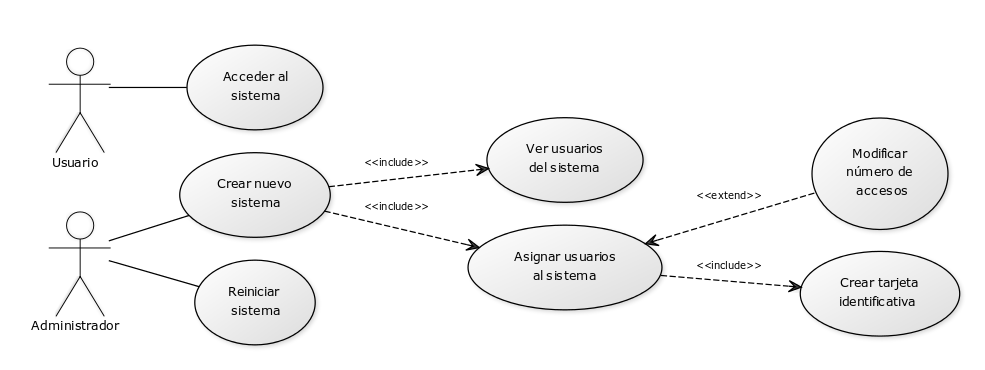
\includegraphics[width=1\textwidth]{./img/usecase1}
  \caption{Casos de uso}
  \label{img:usecase1}
\end{figure}

Los casos de uso, cumpliendo las funcionalidades acordadas con el cliente, se corresponden con los requisitos funcionales de la aplicación y la infraestructura de la aplicación referida en la figura \ref{img:infraestructura}:

\begin{itemize}
\item{Usuario}
	\begin{itemize}
	\item{RF01 - Un usuario, supuesto trabajador de la empresa, poseedor de una tarjeta de identificación proveída por la administración del sistema, es capaz de autenticarse.}
	\end{itemize}
\item{Administrador}
	\begin{itemize}
	\item{RF02 - La administración del sistema define las características del criptosistema que utiliza la aplicación.}
	\item{RF03 - Puede restaurar la información a los valores por defecto.}
	\item{RF04 - Puede ver los usuarios pertenecientes al sistema.}
	\item{RF05 - Es capaz de asignar usuarios al sistema creando las tarjetas identificadores.}
	\item{RF06 - Valida la información recogida de cada tarjeta y sobrescribe con la nueva información acorde al criptosistema empleado.}
	\end{itemize}
\end{itemize}

Como requisitos no funcionales se definen principalmente los siguientes:

\begin{itemize}
\item{Plataforma: Se utiliza un dispositivo \textit{Android} que cumpla las funciones de administración y validación.}
\item{Criptosistema: Compuesto por criptografía con curvas elípticas de alta seguridad y el sistema \textit{SKEY} para validaciones de un solo uso (\textit{véase apartado sobre \ref{App:Seguridad y criptología} la seguridad de la aplicación}). La plataforma utilizada puede modificar la curva elíptica implementada por el criptosistema.}
\item{Elementos identificativos: Las tarjetas NFC contendrán la información asignada por el criptosistema. La información se escribirá a la hora e la asignación del usuario al sitema o en el momento de una validación correcta.}
\end{itemize}

Las definiciones en profundidad de estos casos de uso se muestran a continuación.

\begin{usecase}
\addtitle{Caso de uso}{Acceder al sistema} 
%Primary Actor: Calls on the system to deliver its services.
\addfield{Actor principal:}{Usuario/Empleado}

%Stakeholders and Interests: Who cares about this use case and what do they want?
\additemizedfield{\textit{Stakeholders} e interesados:}{
	\item Usuario/Empleado: Validar su identidad para acceder a las instalaciones de la empresa.
	\item Empresa: Autenticar inequívocamente a quienes acceden a emplazamiento de la empresa.
}
%Preconditions: What must be true on start and worth telling the reader?
\additemizedfield{Precondiciones:}{
\item El usuario dispone de una tarjeta NFC creada por el sistema.
\item La aplicación se encuentra instalada en el dispositivo \textit{Android}.
\item La aplicación posee un sistema de seguridad desplegado.
\item El dispositivo cuenta con la tecnología NFC y en estado activo.
}
%when multiple
%\additemizedfield{Preconditions:}{} 

%Postconditions: What must be true on successful completion and worth telling the reader
\additemizedfield{Postcondiciones:}{
\item La aplicación valida el contenido de la tarjeta NFC e informa al usuario del resultado.
\item La aplicación reescribe la tarjeta NFC preparándola para su siguiente uso.
}
%when multiple
%\additemizedfield{Preconditions:}{}

%Main Success Scenario: A typical, unconditional happy path scenario of success.
\addscenario{Escenario principal de éxito:}{
	\item[1] Se inicia el dispositivo.
	\item[2] Se aproxima la tarjeta NFC al terminal para la lectura del contenido.
	\item[3] La aplicación muestra un mensaje de validación confirmada y escribe el contenido oportuno para la próxima ocasión.
}

%Extensions: Alternate scenarios of success or failure.
\addscenario{Extensiones:}{
	\item[1] Se inicia la aplicación:
		\begin{enumerate}
		\item[1.] Se despliega el menú
		\item[2.] Se selecciona la opción Verificar NFC
		\end{enumerate}
	\item[2] Se aproxima una tarjeta NFC que no es del tipo correcto o el contenido es vacío:
		\begin{enumerate}
		\item[1.] La aplicación muestra un mensaje de aviso
		\item[2.] Vuelta al paso 1 del escenario principal.
		\end{enumerate}
	\item[3] Datos de la tarjeta NFC incorrectos:
		\begin{enumerate}
		\item[1.] El sistema muestra el de validación incorrecta.
		\item[2.] Vuelta al paso 1 del escenario principal.
		\end{enumerate}
}

%Frequency of Occurrence: Influences investigation, testing and timing of implementation.
\addfield{Frecuencia de ocurrencia:}{Cada vez que un usuario del sistema desee autenticarse mediante su tarjeta NFC.}

\end{usecase}

\begin{usecase}
\addtitle{Caso de uso}{Crear nuevo sistema} 
%Primary Actor: Calls on the system to deliver its services.
\addfield{Actor principal:}{Administrador}

%Stakeholders and Interests: Who cares about this use case and what do they want?
\additemizedfield{\textit{Stakeholders} e interesados:}{
	\item Administrador: Definir un nuevo sistema de seguridad suplantando al actual.
}
%Preconditions: What must be true on start and worth telling the reader?
\additemizedfield{Precondiciones:}{
\item La aplicación se encuentra instalada en el dispositivo \textit{Android}.
\item La aplicación posee un sistema de seguridad desplegado.
}
%when multiple
%\additemizedfield{Preconditions:}{} 

%Postconditions: What must be true on successful completion and worth telling the reader
\additemizedfield{Postcondiciones:}{
\item La aplicación implementa una nueva definición del sistema utilizado. Cambiando las características de la curva elíptica a emplear en el futuro.
\item No hay nuevos usuarios asignados en el nuevo sistema.
}
%when multiple
%\additemizedfield{Preconditions:}{}

%Main Success Scenario: A typical, unconditional happy path scenario of success.
\addscenario{Escenario principal de éxito:}{
	\item[1] Se inicia el dispositivo.
	\item[2] Se inicia la aplicación.
	\item[3] Se abre el menú lateral.
	\item[4] Se selecciona la opción Despliegue.
	\item[5] Se selecciona la definición de una curva elíptica utilizando el desplegable.
	\item[6] Se pulsa en crear.
	\item[7] Se muestra un cuadro de confirmación.	
	\item[8] Tras aceptar, se prepara el sistema para asignar nuevos usuarios con la nueva definición.	
}

%Extensions: Alternate scenarios of success or failure.
\addscenario{Extensiones:}{
	\item[4] Se pasa directamente al punto 6 del escenario principal:
		\begin{enumerate}
		\item[1.] La definición por elegida es la listada por defecto.
		\end{enumerate}
	\item[7] Pulsar en Cancelar:
		\begin{enumerate}
		\item[1.] Se cierra el cuadro de confirmación.
		\item[2.] Se vuelve al punto 4 del escenario principal.
		\end{enumerate}
	\item[8] Error en la creación del sistema:
		\begin{enumerate}
		\item[1.] Se muestra un mensaje de error
		\item[2.] Vuelta al paso 4 del escenario principal.
		\end{enumerate}
}

%Frequency of Occurrence: Influences investigation, testing and timing of implementation.
\addfield{Frecuencia de ocurrencia:}{Cada vez que se desee reiniciar los datos de la aplicación con una nueva definición de seguridad.}

\end{usecase}

\begin{usecase}
\addtitle{Caso de uso}{Reiniciar sistema} 
%Primary Actor: Calls on the system to deliver its services.
\addfield{Actor principal:}{Administrador}

%Stakeholders and Interests: Who cares about this use case and what do they want?
\additemizedfield{\textit{Stakeholders} e interesados:}{
	\item Desarrollador: Revertir todos los cambios respecto a la definición de ejemplo.
}
%Preconditions: What must be true on start and worth telling the reader?
\additemizedfield{Precondiciones:}{
\item La aplicación se encuentra instalada en el dispositivo \textit{Android}.
\item La aplicación posee un sistema desplegado.
}
%when multiple
%\additemizedfield{Preconditions:}{} 

%Postconditions: What must be true on successful completion and worth telling the reader
\additemizedfield{Postcondiciones:}{
\item La aplicación recupera la implementación del sistema de ejemplo.
}
%when multiple
%\additemizedfield{Preconditions:}{}

%Main Success Scenario: A typical, unconditional happy path scenario of success.
\addscenario{Escenario principal de éxito:}{
	\item[1] Se inicia el dispositivo.
	\item[2] Se inicia la aplicación.
	\item[3] Se abre el menú lateral.
	\item[4] Se selecciona la opción Despliegue.
	\item[5] Se selecciona la pestaña de Base de datos.
	\item[6] Se pulsa en el botón Restaurar Base de Datos.
	\item[7] Se muestra un cuadro de confirmación.	
	\item[8] Tras aceptar, se recupera el sistema de ejemplo inicial.
}

%Extensions: Alternate scenarios of success or failure.
\addscenario{Extensiones:}{
	\item[7] Pulsar en Cancelar:
		\begin{enumerate}
		\item[1.] Se cierra el cuadro de confirmación.
		\item[2.] Se vuelve al punto 5 del escenario principal.
		\end{enumerate}
	\item[8] Error en la restauración del sistema:
		\begin{enumerate}
		\item[1.] Se muestra un mensaje de error
		\item[2.] Vuelta al paso 5 del escenario principal.
		\end{enumerate}
}

%Frequency of Occurrence: Influences investigation, testing and timing of implementation.
\addfield{Frecuencia de ocurrencia:}{En cualquier momento que se desee.}

\end{usecase}

\begin{usecase}
\addtitle{Caso de uso}{Ver usuarios del sistema} 
%Primary Actor: Calls on the system to deliver its services.
\addfield{Actor principal:}{Administrador}

%Stakeholders and Interests: Who cares about this use case and what do they want?
\additemizedfield{\textit{Stakeholders} e interesados:}{
	\item Administrador: Listar la información de los usuarios del sistema.
}
%Preconditions: What must be true on start and worth telling the reader?
\additemizedfield{Precondiciones:}{
\item La aplicación se encuentra instalada en el dispositivo \textit{Android}.
\item La aplicación posee un sistema desplegado.
}
%when multiple
%\additemizedfield{Preconditions:}{} 

%Postconditions: What must be true on successful completion and worth telling the reader
\additemizedfield{Postcondiciones:}{
\item La aplicación muestra los usuarios activos del sistema .
}
%when multiple
%\additemizedfield{Preconditions:}{}

%Main Success Scenario: A typical, unconditional happy path scenario of success.
\addscenario{Escenario principal de éxito:}{
	\item[1] Se inicia el dispositivo.
	\item[2] Se inicia la aplicación.
	\item[3] Abrir el menú lateral.
	\item[4] Seleccionar la opción Ver Usuarios.
	\item[5] Se lista la tabla con la información de seguridad de los usuarios activos en el sistema.
}

%Extensions: Alternate scenarios of success or failure.
\addscenario{Extensiones:}{
	\item[4] No hay usuarios activos en el sistema:
		\begin{enumerate}
		\item[1.] Se muestra un mensaje indicándolo
		\end{enumerate}
}

%Frequency of Occurrence: Influences investigation, testing and timing of implementation.
\addfield{Frecuencia de ocurrencia:}{En cualquier momento que se desee.}

\end{usecase}

\begin{usecase}
\addtitle{Caso de uso}{Asignar usuarios al sistema} 
%Primary Actor: Calls on the system to deliver its services.
\addfield{Actor principal:}{Administrador}

%Stakeholders and Interests: Who cares about this use case and what do they want?
\additemizedfield{\textit{Stakeholders} e interesados:}{
	\item Administrador: Crear (escribir) tarjetas NFC para autenticar dentro del sistema generado a un empleado de la empresa.
	\item Usuario/Empleado: Obtener una tarjeta NFC con el contenido adecuado.
}
%Preconditions: What must be true on start and worth telling the reader?
\additemizedfield{Precondiciones:}{
\item La aplicación se encuentra instalada en el dispositivo \textit{Android}.
\item La aplicación posee un sistema desplegado.
\item El dispositivo cuenta con la tecnología NFC y en estado activo.
\item La tarjeta NFC objetivo contiene información por defecto (no está vacía) para evitar fallos de escritura.
\item La aplicación dispone de un listado de usuarios generales de la empresa.
}
%when multiple
%\additemizedfield{Preconditions:}{} 

%Postconditions: What must be true on successful completion and worth telling the reader
\additemizedfield{Postcondiciones:}{
\item Se vuelca el contenido de autenticación de un usuario recién añadido al sistema a una tarjeta NFC.
}
%when multiple
%\additemizedfield{Preconditions:}{}

%Main Success Scenario: A typical, unconditional happy path scenario of success.
\addscenario{Escenario principal de éxito:}{
	\item[1] Se inicia el dispositivo.
	\item[2] Se inicia la aplicación.
	\item[3] Pulsar en abrir el menú lateral.
	\item[4] Seleccionar la opción Nuevo Usuario.
	\item[5] Seleccionar un usuario que no esté asignado al sistema actual.
	\item[6] Pulsar el botón Continuar.
	\item[7] Se muestra un mensaje de confirmación.	
	\item[8] Un mensaje de de información indica que la aplicación está preparada para escribir en la tarjeta. Se acerca la tarjeta para escribir.
	\item[9] La aplicación ha escrito correctamente la información en la tarjeta NFC.
}

%Extensions: Alternate scenarios of success or failure.
\addscenario{Extensiones:}{
	\item[7] Pulsar en Cancelar:
		\begin{enumerate}
		\item[1.] Se cierra el cuadro de confirmación.
		\item[2.] Se vuelve al punto 5 del escenario principal.
		\end{enumerate}
	\item[8] Fallo al escribir:
		\begin{enumerate}
		\item[1.] Se muestra un mensaje indicando el fallo de escritura.
		\item[2.] No se añade el usuario al nuevo sistema.
		\item[3.] Se prepara la escritura nuevamente, paso al punto 8 del escenario principal.		
		\end{enumerate}		
}

%Frequency of Occurrence: Influences investigation, testing and timing of implementation.
\addfield{Frecuencia de ocurrencia:}{Cuando se requiera asignar un usuario al sistema.}

\end{usecase}

\section{Diseño y aspecto}
\label{App:Diseño y aspecto}

La aplicación cuenta con un contenedor principal que ocupa la visión principal del dispositivo. En la parte superior dispone de barra principal de la aplicación que contiene el título de cada apartado y un acceso al menú. El menú se muestra desde la parte izquierda ocupando gran parte de la pantalla. Muestra una cabecera de menú y el listado de apartados de la aplicación.
\\\\
Principalmente estos elementos son los que definen el diseño principal de la aplicación. La disposición sigue las normas básicas para el diseño de una aplicación \textit{Android} utilizando \textit{material desing} de \textit{Google}\cite{materialDesign}. Tanto la sombra de la barra principal, la sombra de fondo al mostrar el menú, el menú que se superpone a la barra principal y por debajo de los indicadores del dispositivo, la organización de los elementos del menú, el espaciado entre los elementos, la iconografía y demás elementos siguen en su mayoría las indicaciones de \textit{material desing}. En la figura \ref{img:designElements} se puede apreciar gran parte de estos elementos de diseño.

%\begin{figure}[H]
%  \centering
%  \csubfloat{\includegraphics[width=0.35\textwidth]{./img/pantallaPrincipal}}
%  \centerhfill
%  \csubfloat{\includegraphics[width=0.35\textwidth]{./img/menuDesplegado}}
%  \hspace*{\fill}
%  \caption{Elementos de diseño: Muestra de la disposición espacial del menú y estructura básica de la aplicación}
%  \label{img:designElements}
%\end{figure}

\begin{figure}[H]
\centering
	\begin{subfigure}{0.4\textwidth}
		\centering
		\includegraphics[scale=0.45]{./img/pantallaPrincipal}
    \end{subfigure}          
    \qquad\qquad\qquad  % spacing between the subfigures
    \begin{subfigure}{0.4\textwidth}  
       \centering
       \includegraphics[scale=0.45]{./img/menuDesplegado}
    \end{subfigure}   
  \caption{Elementos de diseño: Muestra de la disposición espacial del menú y estructura básica de la aplicación}
  \label{img:designElements}
\end{figure}

Es oportuno mencionar la paleta de colores utilizada, tanto para el fondo como para las acentuaciones o el color primario y su homónimo oscuro : 

\begin{itemize}
\item{Color primario: \#009688 .}
\item{Color primario oscuro: \#37474f .}
\item{Color acentuado: \#ff4081 .}
\item{Color base principal: \#367cd3 .}
\end{itemize}

Se han elegido manteniendo la relación de colores de \textit{material desing} y siguiendo normas conocidas de \textit{marketing} y presentación de elementos visuales a consumidores. En estas normas y patrones es común observar que, por ejemplo, el color rojo implica pasión, efervescencia, impulso; ideal para representar ciertos elementos y estimular sensaciones acordes. Nótese que en la mayoría de marcas de comida, el color rojo predomina, ya que lo hace más apetecible al subconsciente humano y predispone al potencial consumidor a querer hacerse con ello. 
\\\\
Siguiendo el mismo ejemplo, el verde en marcas de alimentos se utiliza para representa lo natural, la limpieza y frescura; muy empleado en marcas ecológicas. El color base de la aplicación es el azul (hex:\#367cd3); representa la serenidad, responsabilidad, sinceridad y verdad; apto para ser acogedor y mostrar fiabilidad. Es deliberado el uso de este color al igual que también lo es en la mayoría de las redes sociales. Buscan ganarse la confianza del usuario y dar un ambiente en el que se tenga una experiencia relajante y confortable. Por todo esto, el azul acerca la seguridad del criptosistema utilizado. Para más información sobre la evaluación de elementos visuales para las interfaces de usuario ver \cite{coloresStone}.

\section{Seguridad y criptología}
\label{App:Seguridad y criptología}

La seguridad utilizada se basa en la criptología con curvas elípticas. Para la implementación del criptosistema se han utilizado las clases de la librería \textit{Bouncy Castle} y una interfaz \textit{AppEllipticCurveI} a implementar con los métodos necesarios para la aplicación.
\\\\
El flujo se simplifica básicamente en asignar a los usuarios del sistema un punto $P$ aleatorio en una curva elíptica dentro de un campo finito $G(F(2^m))$. Las curvas están delimitadas por un conjunto de nombres de curvas ya definidas que cumplen ciertas características de seguridad (orden de la curva de más de 130 \textit{bits}) y capacidad objetivo (codificaciones no superiores a la capacidad de las tarjetas NFC). Las curvas siguen diferentes estándares y se cargan en función del nombre que se les atribuye, el listado de las curvas disponibles se puede observar en \cite{bouncyCastleCurves} dentro de las correspondientes a los campos $F(2^m)$.
\\\\
Los puntos $P$ obtenidos se multiplican por una variable aleatoria privada $k$ de 160 \textit{bits} de tamaño obteniendo $kP$. Siguiendo el método \textit{SKEY}, se multiplica el resultado $kP$ tantas veces como usos se hayan indicado a la hora de la creación del punto $P$ (\textit{véase el apartado de la aplicación \ref{App:AD:Nuevo usuario} sobre la creación de usuarios}). Con ello se computa el valor $QkP$ que es un punto en la curva. Computar $kP$ es sencillo, sin embargo, obtener la variable $k$ es computacionalmente muy complejo debido al problema del logaritmo discreto. Para utilizar códigos de un solo uso se computa $Q$ veces la suma de $kP$ para almacenar en la base de datos el punto $(Q+1)kP$ asociado a un usuario de la aplicación; a su vez, se escribe en la tarjeta NFC el valor $QkP$ y el identificador del usuario.
\\\\
A la hora de validar la información de la tarjeta se obtiene la codificación del punto $QkP$ de la tarjeta NFC. A este punto se le añade el punto original $kP$ y se comprueba igual a $(Q+1)kP$ de la base de datos. Si coincide se valida la información con lo que se prepara el código del siguiente uso, que se trata de $(X-1)kP$ y se escribe en la tarjeta (guardando el valor comprobante de $(X+1)kP$ hasta alcanzar $kP$, siendo $X$ el uso actual. Una vez agotados los usos se realiza automáticamente la asignación de un nuevo punto al usuario con los $Q$ usos elegidos originalmente.
\\\\
Se muestra en la figura \ref{img:eci1} y \ref{img:eci2} la estructura de la interfaz mencionada junto a la documentación de cada uno de los métodos que la componen.
 
\begin{figure}[H]
  \centering
  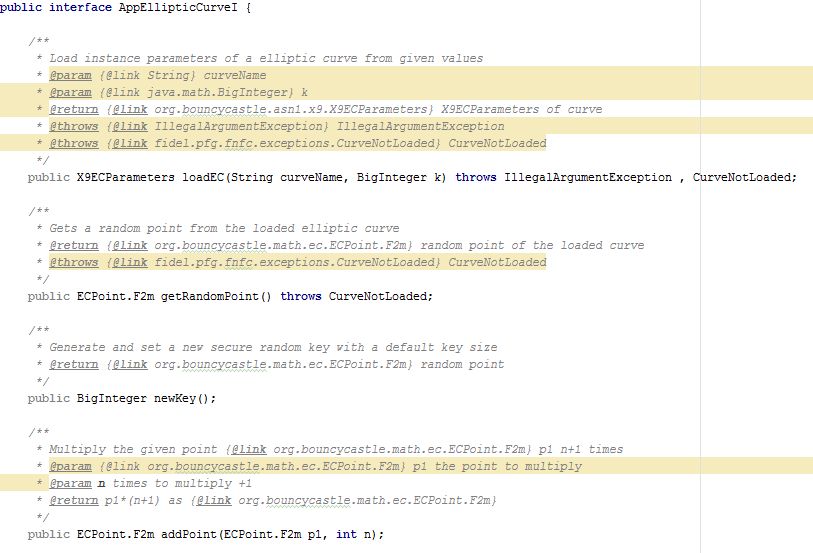
\includegraphics[width=1\textwidth]{./img/eci1}
  \caption{Interfaz AppEllipticCurveI que se implementa en la aplicación (I).}
  \label{img:eci1}
\end{figure}
 
\begin{figure}[H]
  \centering
  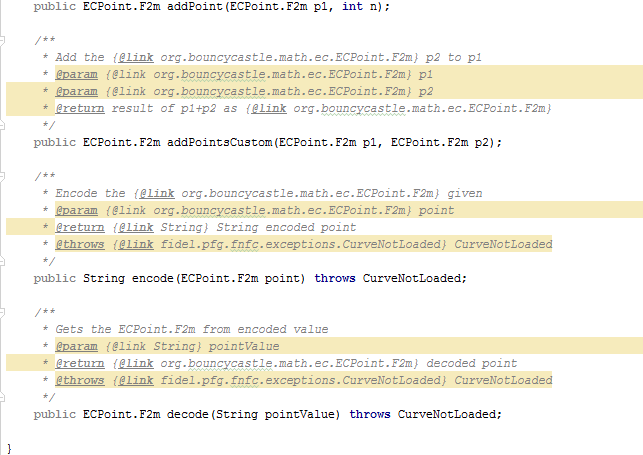
\includegraphics[width=1\textwidth]{./img/eci2}
  \caption{Interfaz AppEllipticCurveI que se implementa en la aplicación (II).}
  \label{img:eci2}
\end{figure}

Dentro de la implementación es oportuno comentar el método \textit{AddCustomPoints} el cuál es la realización por cuenta propia del método de suma de puntos en una curva elíptica en campos finitos del tipo \(GF(2^m)\). La figura \ref{img:addPointsCustom} muestra en detalle la suma implementada.

\begin{figure}[H]
  \centering
  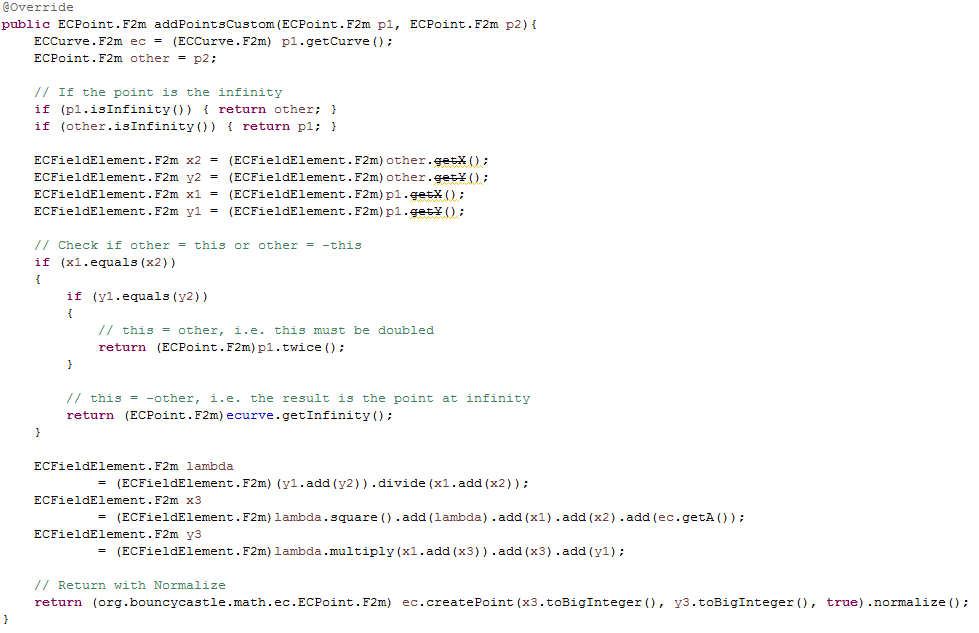
\includegraphics[width=1\textwidth]{./img/addPointsCustom}
  \caption{Suma de puntos implementada en java.}
  \label{img:addPointsCustom}
\end{figure}

Básicamente se divide en dos partes: si los puntos pasados por parámetro son iguales (duplicar el punto) y o si son distintos. Para el caso de puntos iguales, se realiza la llamada al método \textit{twice()} de la clase \textit{ECPoint.F2m} de la librería de \textit{Bouncy Castle}. Por el contrario, en el caso de puntos diferentes, se realiza la suma de puntos en curva elíptica tras unas comprobaciones previas. La fórmula utilizada y comprobada respecto a la realizada internamente por la librería es la siguiente:\\

\begin{center}
$y^2 + xy= x^3 +ax^2 + b\ (mod\ n) \equiv E(G(2^m))$\\
$P=(x_{1},y_{1}), Q=(x_{2},y_{2}), R = P+Q = (x_{3},y_{3})$\\
$P,Q,R\in E(GF(2^m))$\\
$\lambda=(y_{1}+y_{2})/(x_{1}+x_{2})$\\
$x_{3}=\lambda^2+\lambda+x_{1}+x_{2}+a$\\
$y_{3}=\lambda*(x_{1}+x_{3})+x_{3}+y_{1}$\\
\end{center}

La seguridad reside en la privacidad del elemento $k$ difícilmente obtenible pese a que los demás elementos sean públicos gracias a las curvas elípticas en campos finitos y al uso de \textit{SKEY} para utilizar códigos únicos de un solo uso. En el escenario real definido en el apartado \ref{App:Escenario} se utilizaría una comunicación segura de la clave $k$ y otra clave $q$ también empleando curvas elípticas. La idea simplificada es la misma, obtener el valor $k$ de $kP$ es difícilmente computable. En el anexo I \ref{AnexoI} se muestra el código de ejemplo de una comunicación de claves de este tipo. Con ésta implementación se podrían comunicar los valores de forma segura entre los tornos de seguridad y los servidores de comprobación y validación.

\section{Base de datos}
\label{App:Base de datos}

La base de datos, mencionada en el apartado \ref{App:Materiales y tecnologías utilizadas}, es una pequeña \textit{SQLite}. Se utiliza este tipo de base de datos debido a la comodidad y simplicidad con la que trabaja en un proyecto \textit{Android}.
\\\\\
En el escenario virtual de la aplicación, en vez de esta base de datos se utilizaría una centralizada en los servidores de la empresa. Se realizarían conexiones seguras para no comprometer la información a enviar. Sin embargo, ésto no es necesario dentro del ámbito real ya que toda la información que se precisa de los servidores ficticios de la empresa se encuentran dentro de esta pequeña base de datos.
\\\\\
Dentro de esta base de datos se encuentra la información de la curva elíptica implementada y la clave privada asociada (\textit{véase el apartado sobre seguridad y critología \ref{App:Seguridad y criptología}}). También está la información de parte de los usuarios ficticios de la empresa. Por último, se encuentra una tabla referida a la información de cada usuario que compone los datos para poder validar el contenido de cada tarjeta NFC de cada usuario. En la figura \ref{img:database} se observa la distribución de tablas y la relación entre ellas (creado mediante la herramienta online \textit{GenMyModel}\cite{diagramaDBOnline}). Posteriormente en la figura \ref{img:databaseScript} se observa el \textit{script} de creación en lenguaje \textit{SQL}.

\begin{figure}[H]
  \centering
  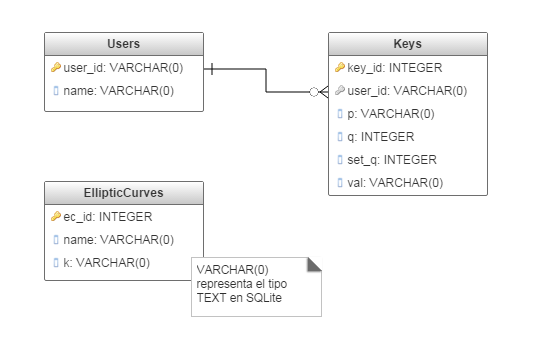
\includegraphics[width=0.7\textwidth]{./img/database}
  \caption{Representación de la base de datos implementada.}
  \label{img:database}
\end{figure}

\begin{figure}[H]
  \centering
  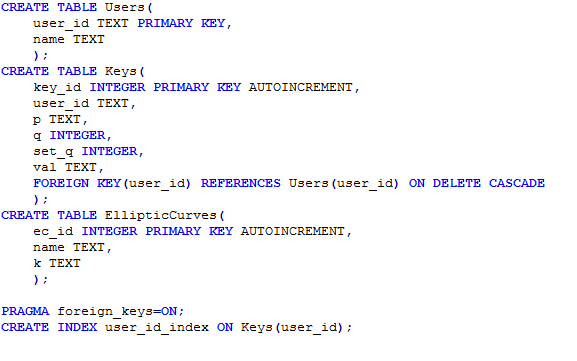
\includegraphics[width=0.8\textwidth]{./img/databaseScript}
  \caption{Script para la creación de la base de datos.}
  \label{img:databaseScript}
\end{figure}

El contenido por defecto del sistema se adecua a la implementación de la curva elíptica \(c2pnb163v1\) (cuyos detalles se pueden encontrar en \cite{definicionCurvasF2M}). La clave por defecto es un número entero de 160 bits que es el siguiente: \(838828326113658401440043399564525405856963575389\). Los distintos valores de los campos \textit{P}, \textit{kP}, \textit{Q} y \textit{Set Q}, \textit{QkP} corresponden con datos válidos del sistema utilizado y de puntos aleatorios de la curva generados bajo la clave mencionada.

\section{Aplicación desarrollada}
\label{App:Aplicación desarrollada}

La aplicación final se compone principalmente de una actividad principal que dispone del menú lateral, la barra superior de acciones y un contenedor que va modificándose en función de la situación. En las siguientes secciones se muestra el contenido, utilización, significado y ejemplos de cada uno de estos apartados que compondrán los datos que se muestran en el contenedor.

\subsection{Inicio}
\label{App:AD:Inicio}

La página de inicio será el contenido por defecto del contenedor. Se presenta el logo de la aplicación junto a unas referencias a la autoría. La figura \ref{img:app:inicio} muestra la visualización en cuestión. También se puede acceder a esta vista desde el menú lateral (\textit{véase sección \ref{App:Menu}}).

\begin{figure}[H]
  \centering
  \includegraphics[width=0.3\textwidth]{./img/app/pantallaPrincipal}
  \caption{Vista de la pantalla por defecto 'Inicio'.}
  \label{img:app:inicio}
\end{figure}

\subsection{Menú}
\label{App:Menu}

Para acceder al menú de la aplicación se puede pulsar en el extremo superior-izquierdo de la pantalla o deslizar el dedo desde el lateral izquierdo hacia el derecho. Se listan las posibles opciones de la aplicación como se observa en la figura \ref{img:app:menuDesplegado}.

\begin{figure}[H]
  \centering
  \subfloat{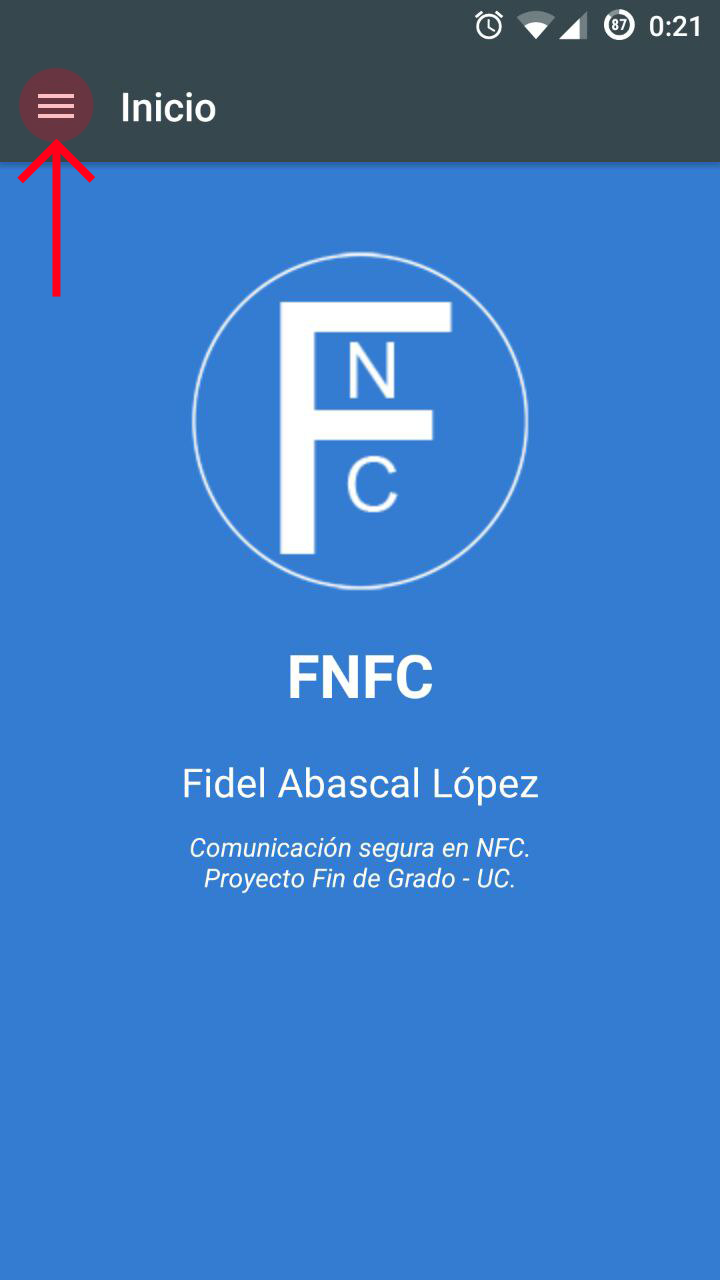
\includegraphics[width=0.35\textwidth]{./img/app/accesoMenu}}
  \null\hfill
  \subfloat{\includegraphics[width=0.35\textwidth]{./img/app/menuDesplegado}}
  \caption{Acceso y vista del menú desplegado}
  \label{img:app:menuDesplegado}
\end{figure}

\subsection{Acerca de}
\label{App:AD:Acerca de}

Como elemento del menú se puede acceder a la pantalla donde se visualiza en el contenedor principal la información relacionada con la aplicación. La figura \ref{img:app:acercaDe} muestra la visualización de esta pantalla.

\begin{figure}[H]
  \centering
  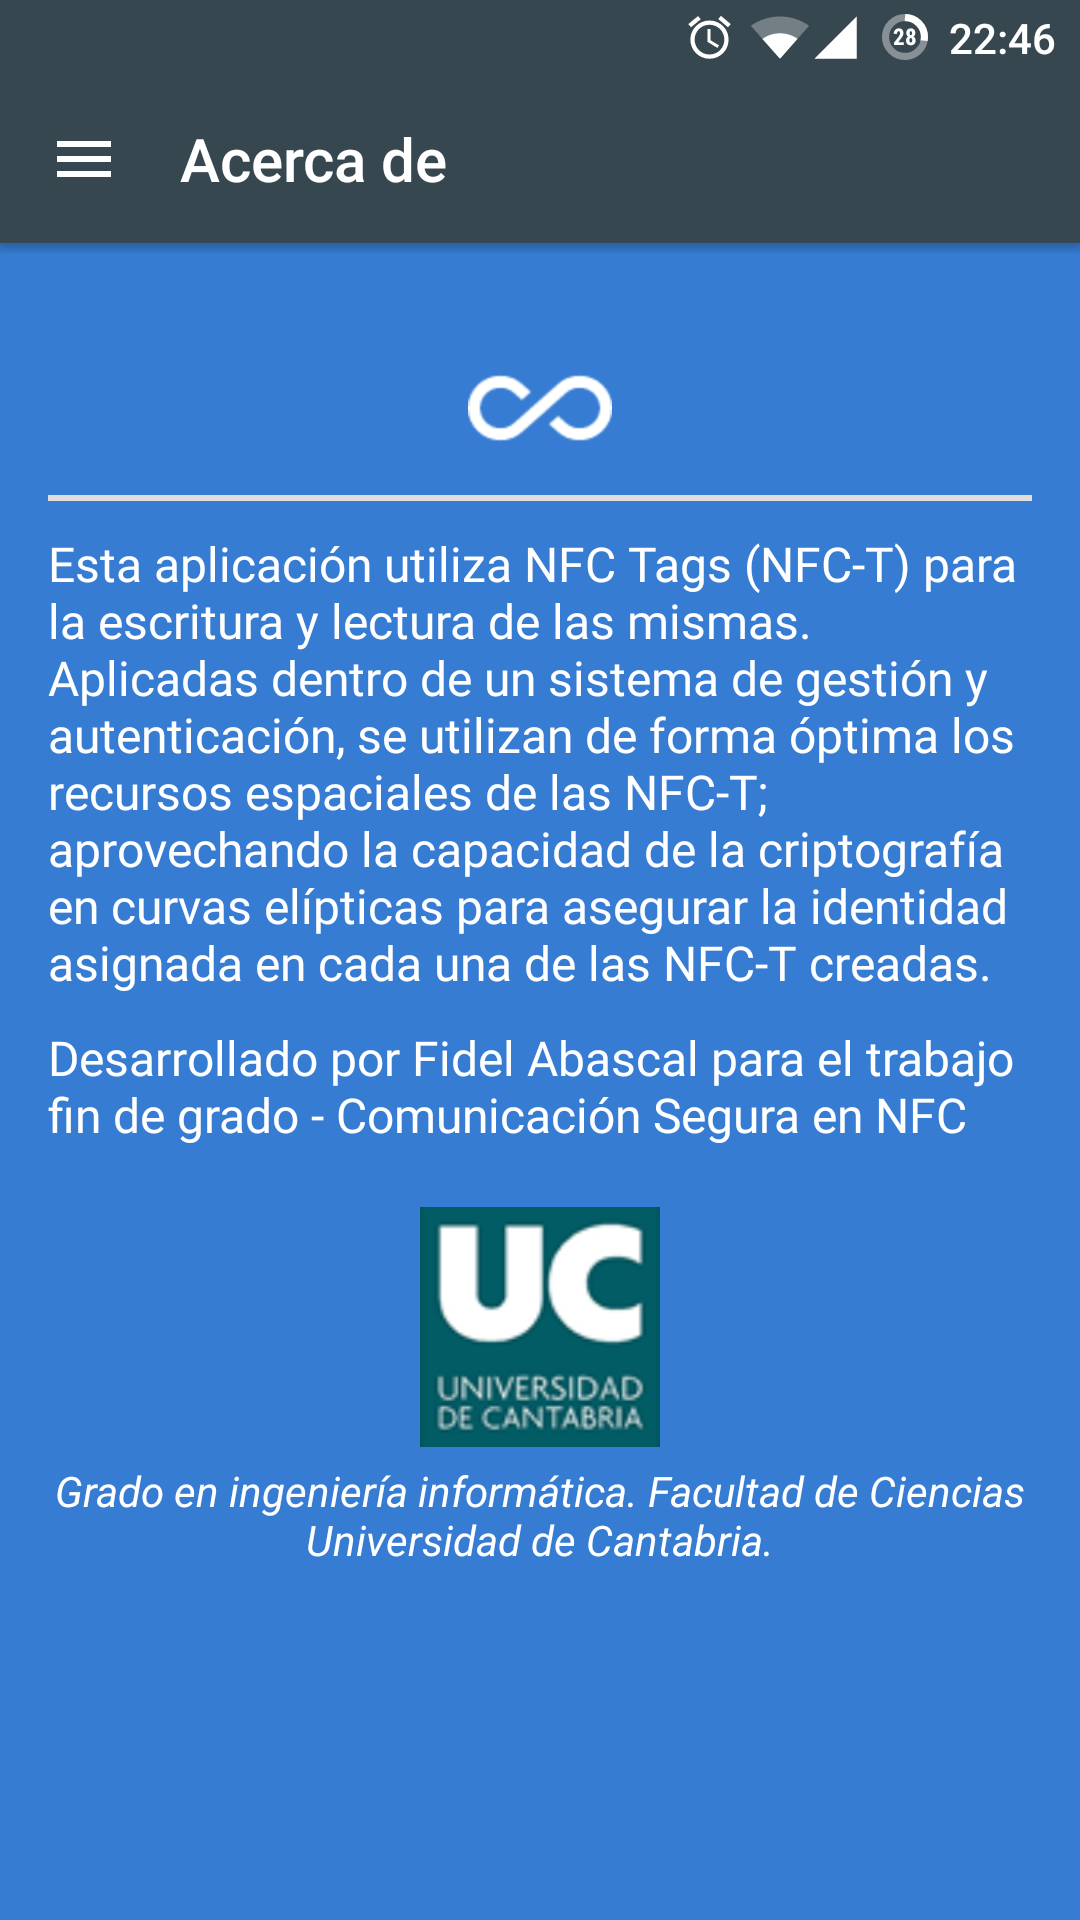
\includegraphics[width=0.3\textwidth]{./img/app/acercaDe}
  \caption{Vista de la pantalla 'Acerca De'.}
  \label{img:app:acercaDe}
\end{figure}  

\subsection{Despliegue}
\label{App:AD:Despliegue}

Accediendo a la parte administrativa de la aplicación desde el menú llamada despliegue. En ella se muestra la pestaña del sistema y de la base de datos que se mostrarán al siguientes secciones.

\subsubsection{Sistema}
\label{App:AD:D:Sistema}

En la pestaña de sistema se muestra una advertencia de desplegar una nueva configuración de seguridad del criptosistema. A su vez, se puede escoger la definición de la curva a implementar antes de crear una nueva. Cuando se pulsa en la creación del nuevo sistema se muestra un mensaje de confirmación previo como se aprecia en la figura \ref{img:app:sistema}.

\begin{figure}[H]
  \centering
  \subfloat{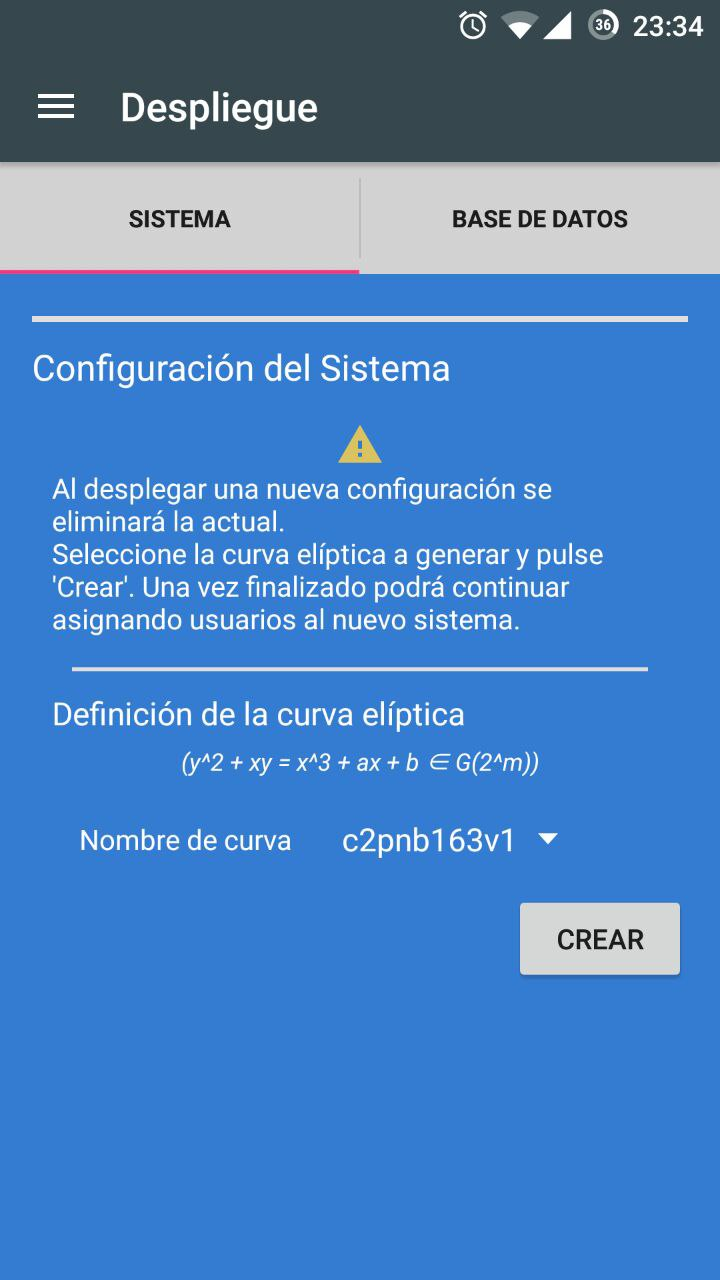
\includegraphics[width=0.35\textwidth]{./img/app/despliegueSistema}}
  \null\hfill
  \subfloat{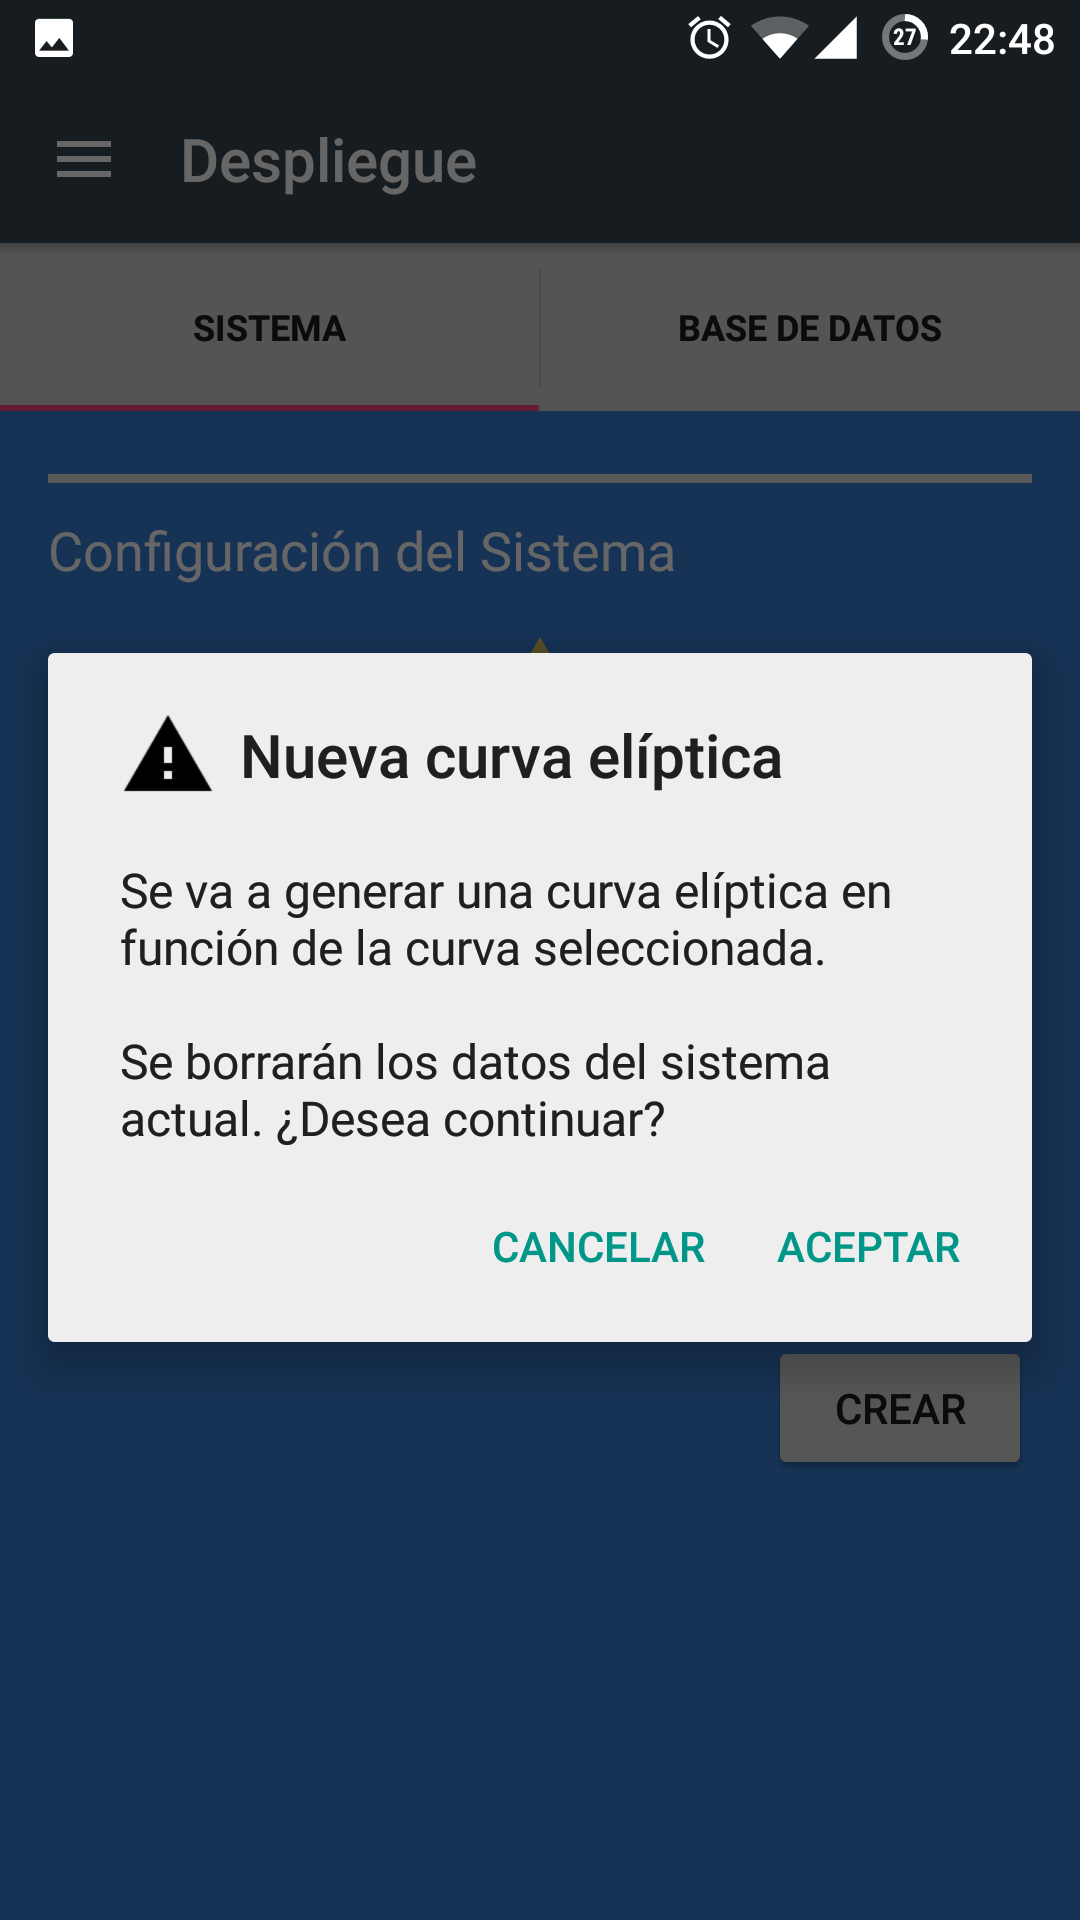
\includegraphics[width=0.35\textwidth]{./img/app/despligueSistemaDialog}}
  \caption{Pantalla de despliegue del sistema.}
  \label{img:app:sistema}
\end{figure}


\subsubsection{Base de datos}
\label{App:AD:D:Base de dtaos}

Otra funcionalidad de la aplicación es la de restaurar la base de datos con los parámetros por defecto. Antes de pulsar en el botón de restauración se pedirá una confirmación, finalizando con un mensaje como se puede observar en las figuras \ref{img:app:baseDatos1} y \ref{img:app:baseDatos2} .

\begin{figure}[H]
  \centering
  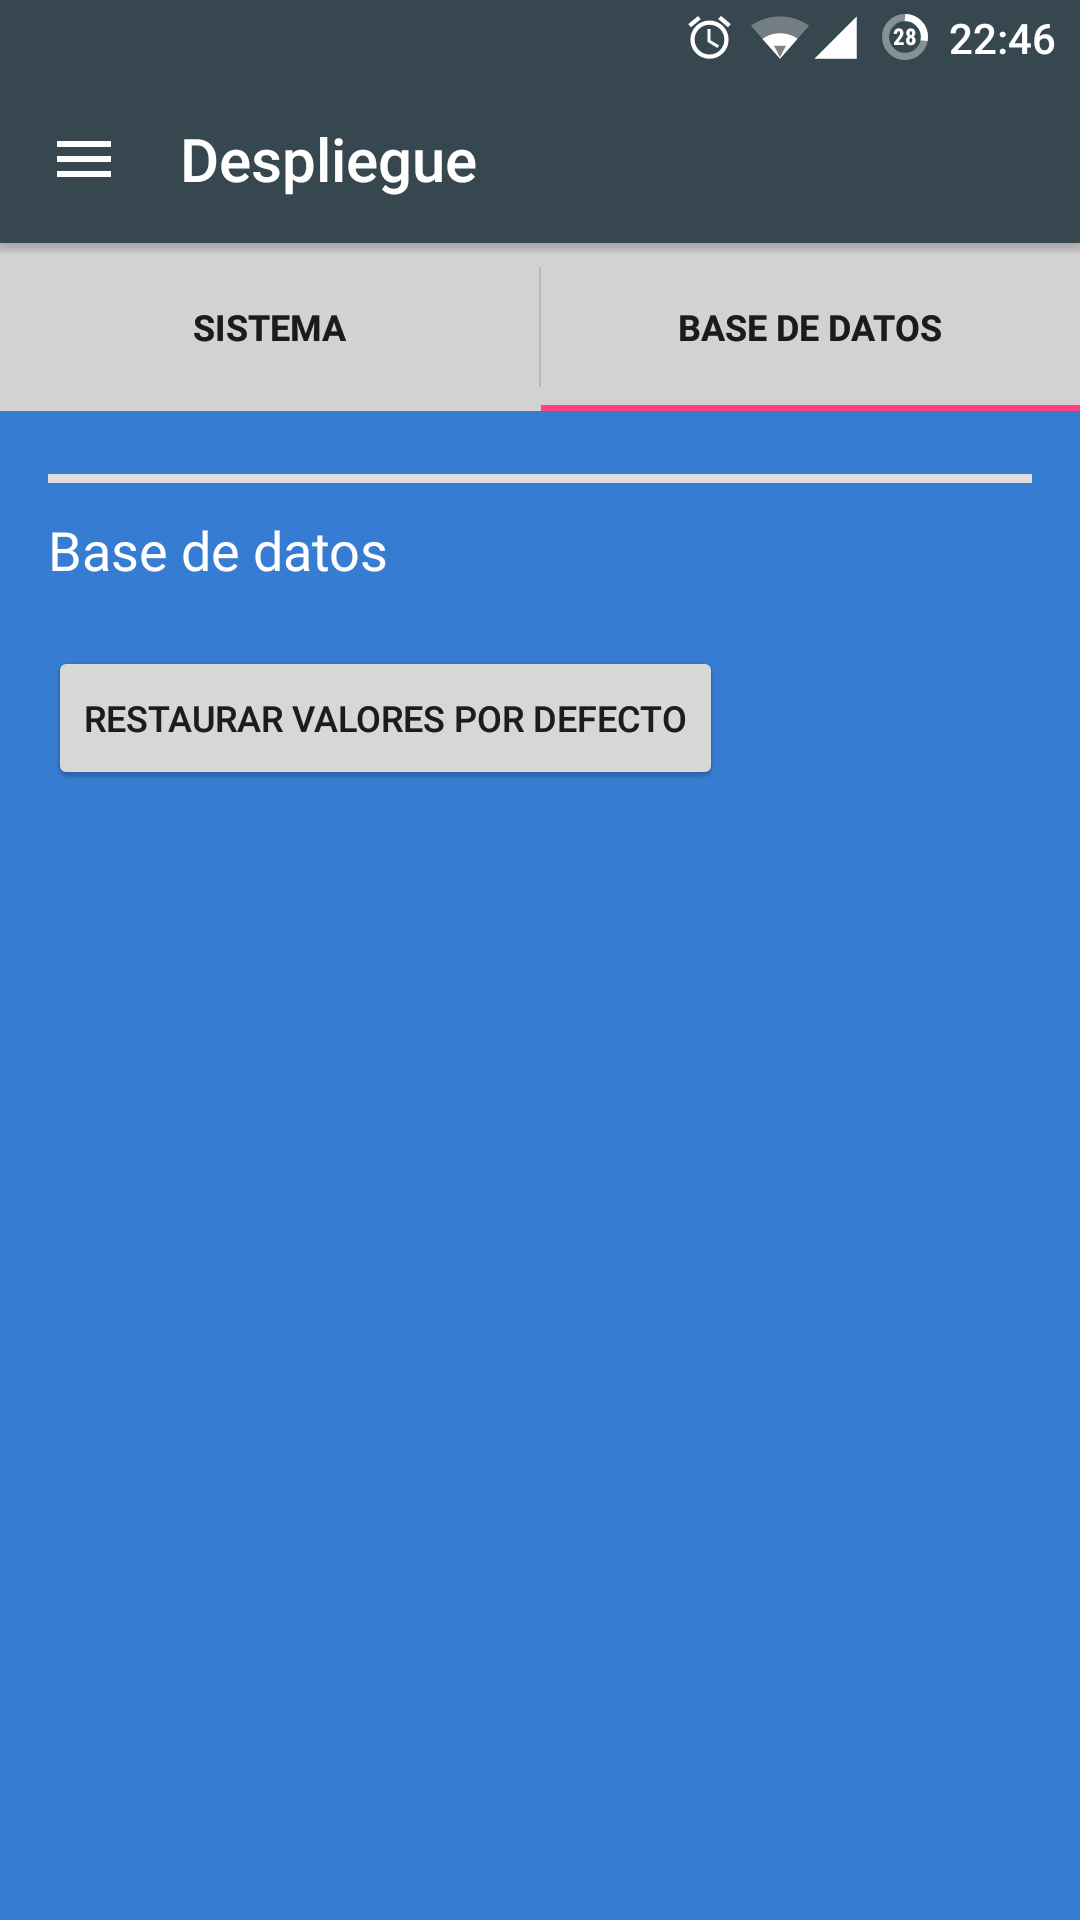
\includegraphics[width=0.3\textwidth]{./img/app/despliegueBaseDeDatos}
  \caption{Pantalla 'Base de Datos'.}
  \label{img:app:baseDatos1}
\end{figure}  

\begin{figure}[H]
  \centering
  \subfloat{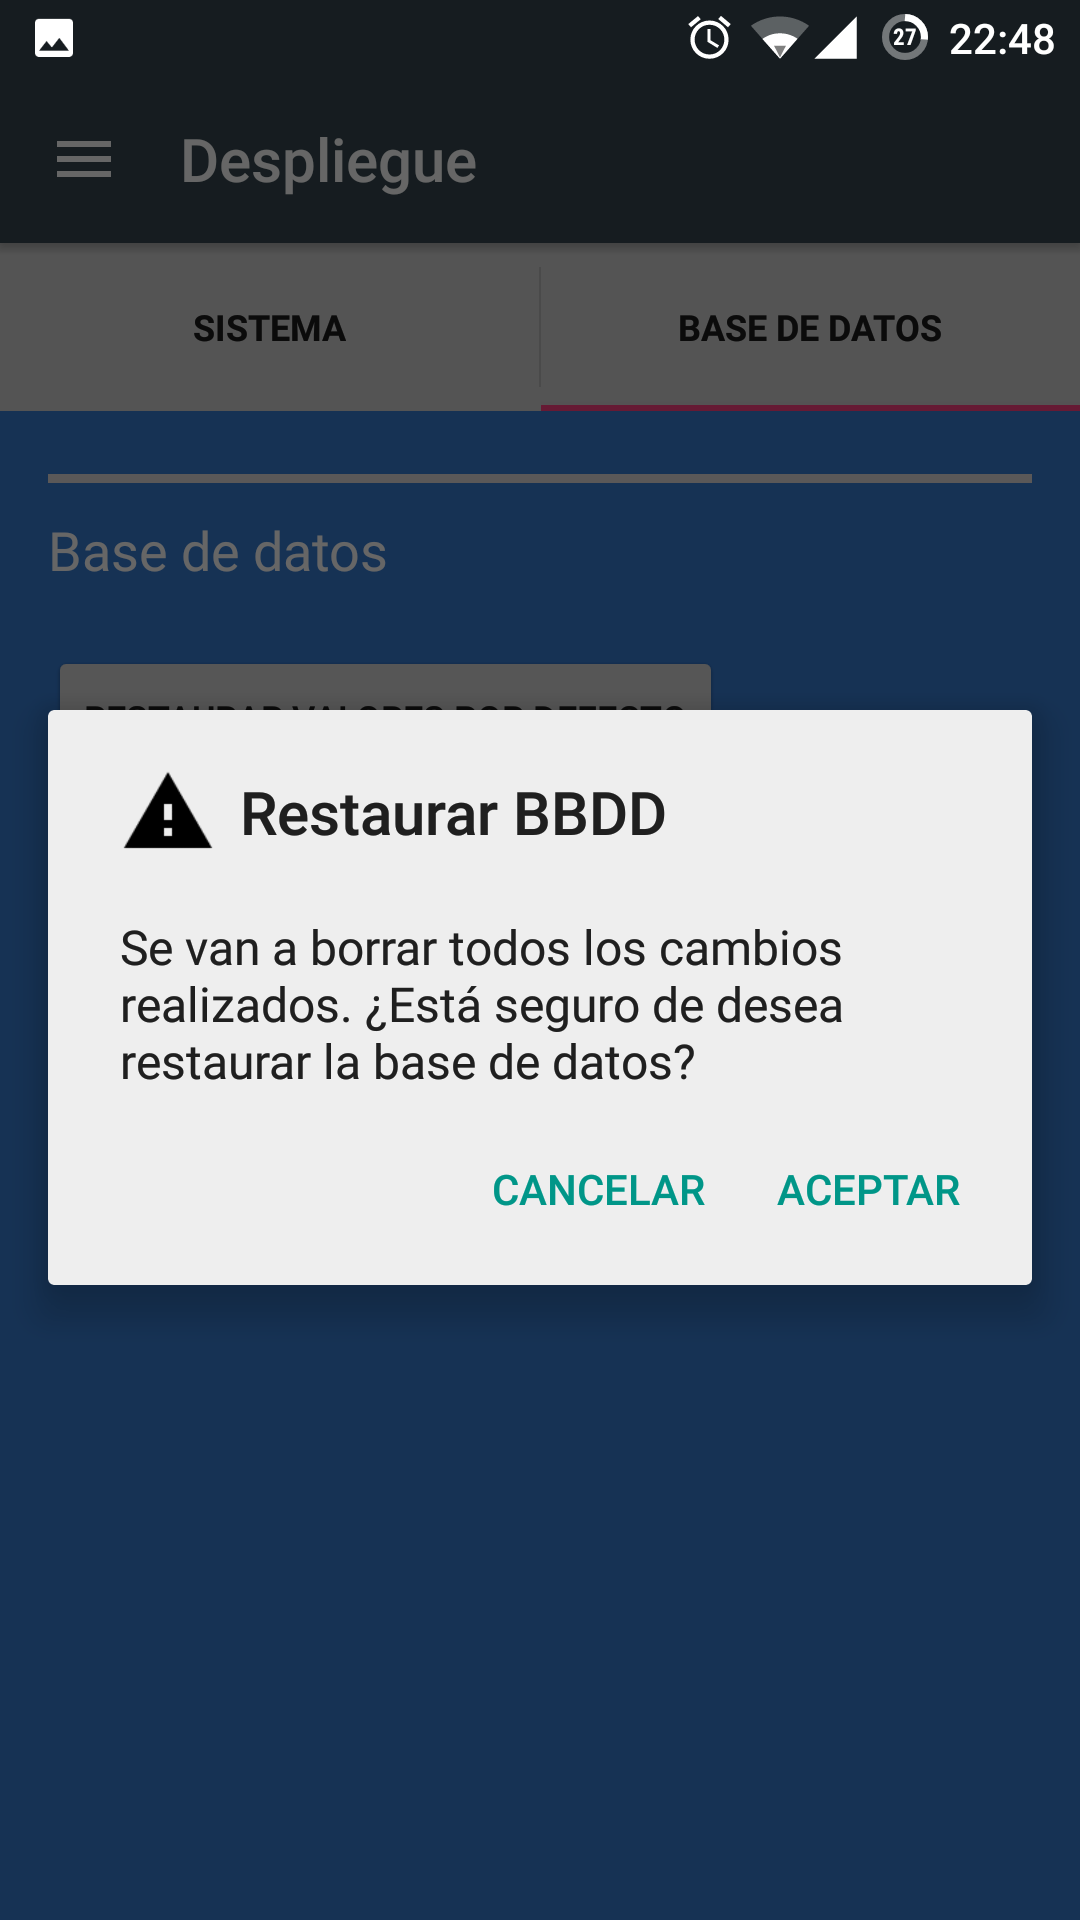
\includegraphics[width=0.35\textwidth]{./img/app/despliegueBaseDeDatosDialog}}
  \null\hfill
  \subfloat{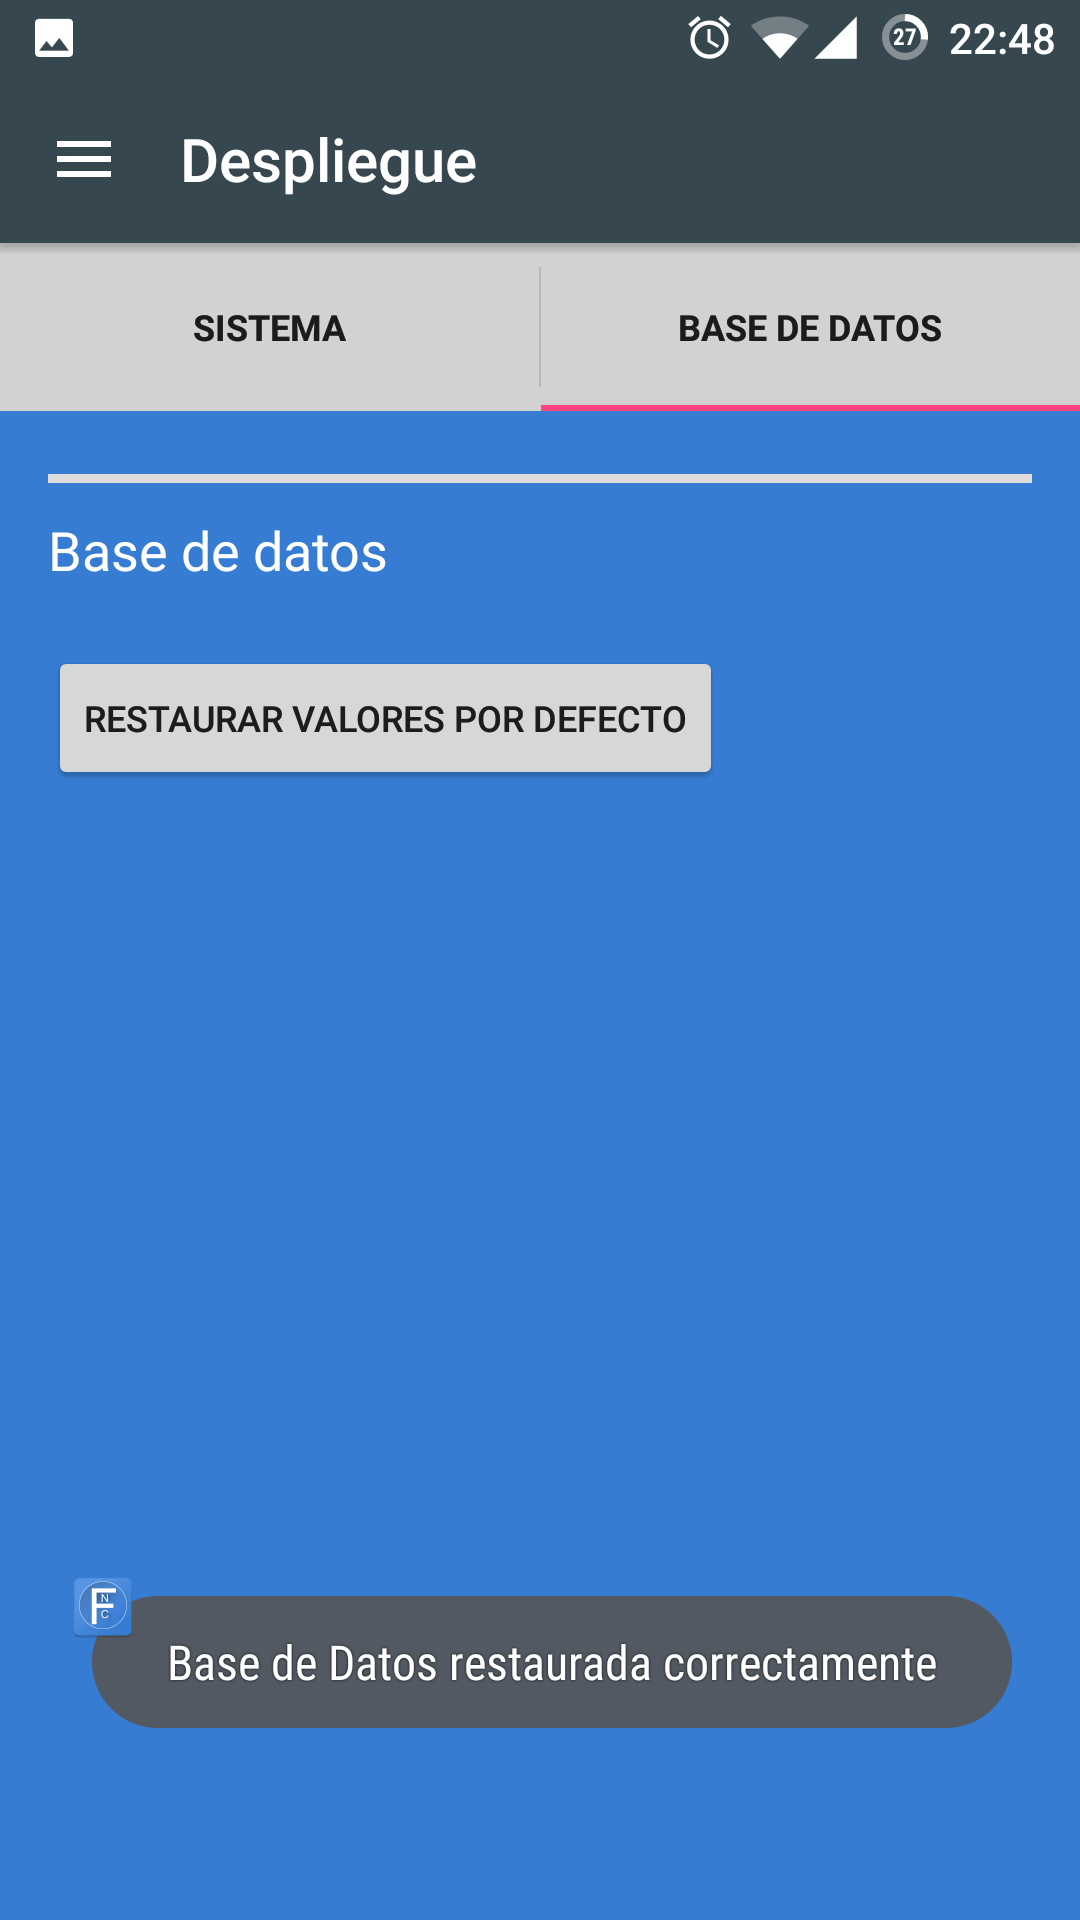
\includegraphics[width=0.35\textwidth]{./img/app/despliegueBaseDeDatosMensaje}}
  \caption{Restauración de los datos por defecto.}
  \label{img:app:baseDatos2}
\end{figure}

\subsection{Nuevo usuario}
\label{App:AD:Nuevo usuario}

Mediante el menú se accede a la pantalla de creación de nuevo usuario. En esta pantalla se listará en un desplegable los usuarios disponibles (no asignados al sistema actual) y un \textit{spinner} para seleccionar el número de usos que dispondrá el usuario por punto $P$ (ver el apartado de seguridad y criptología \ref{App:Seguridad y criptología}). Cuando se hayan seleccionado los datos se muestra un mensaje de confirmación y aviso para tener a mano la tarjeta NFC en la que se va a grabar la información. La tarjeta deberá seguir el requisito de no estar vacía. La próxima vez que se acerque una tarjeta al terminal escribirá el contenido. Al escribir en la tarjeta se mostrará la pantalla de verificación. En las siguientes figuras \ref{img:app:nuevoUsuario1} y \ref{img:app:nuevoUsuario2} se puede apreciar el funcionamiento.

\begin{figure}[H]
  \centering
  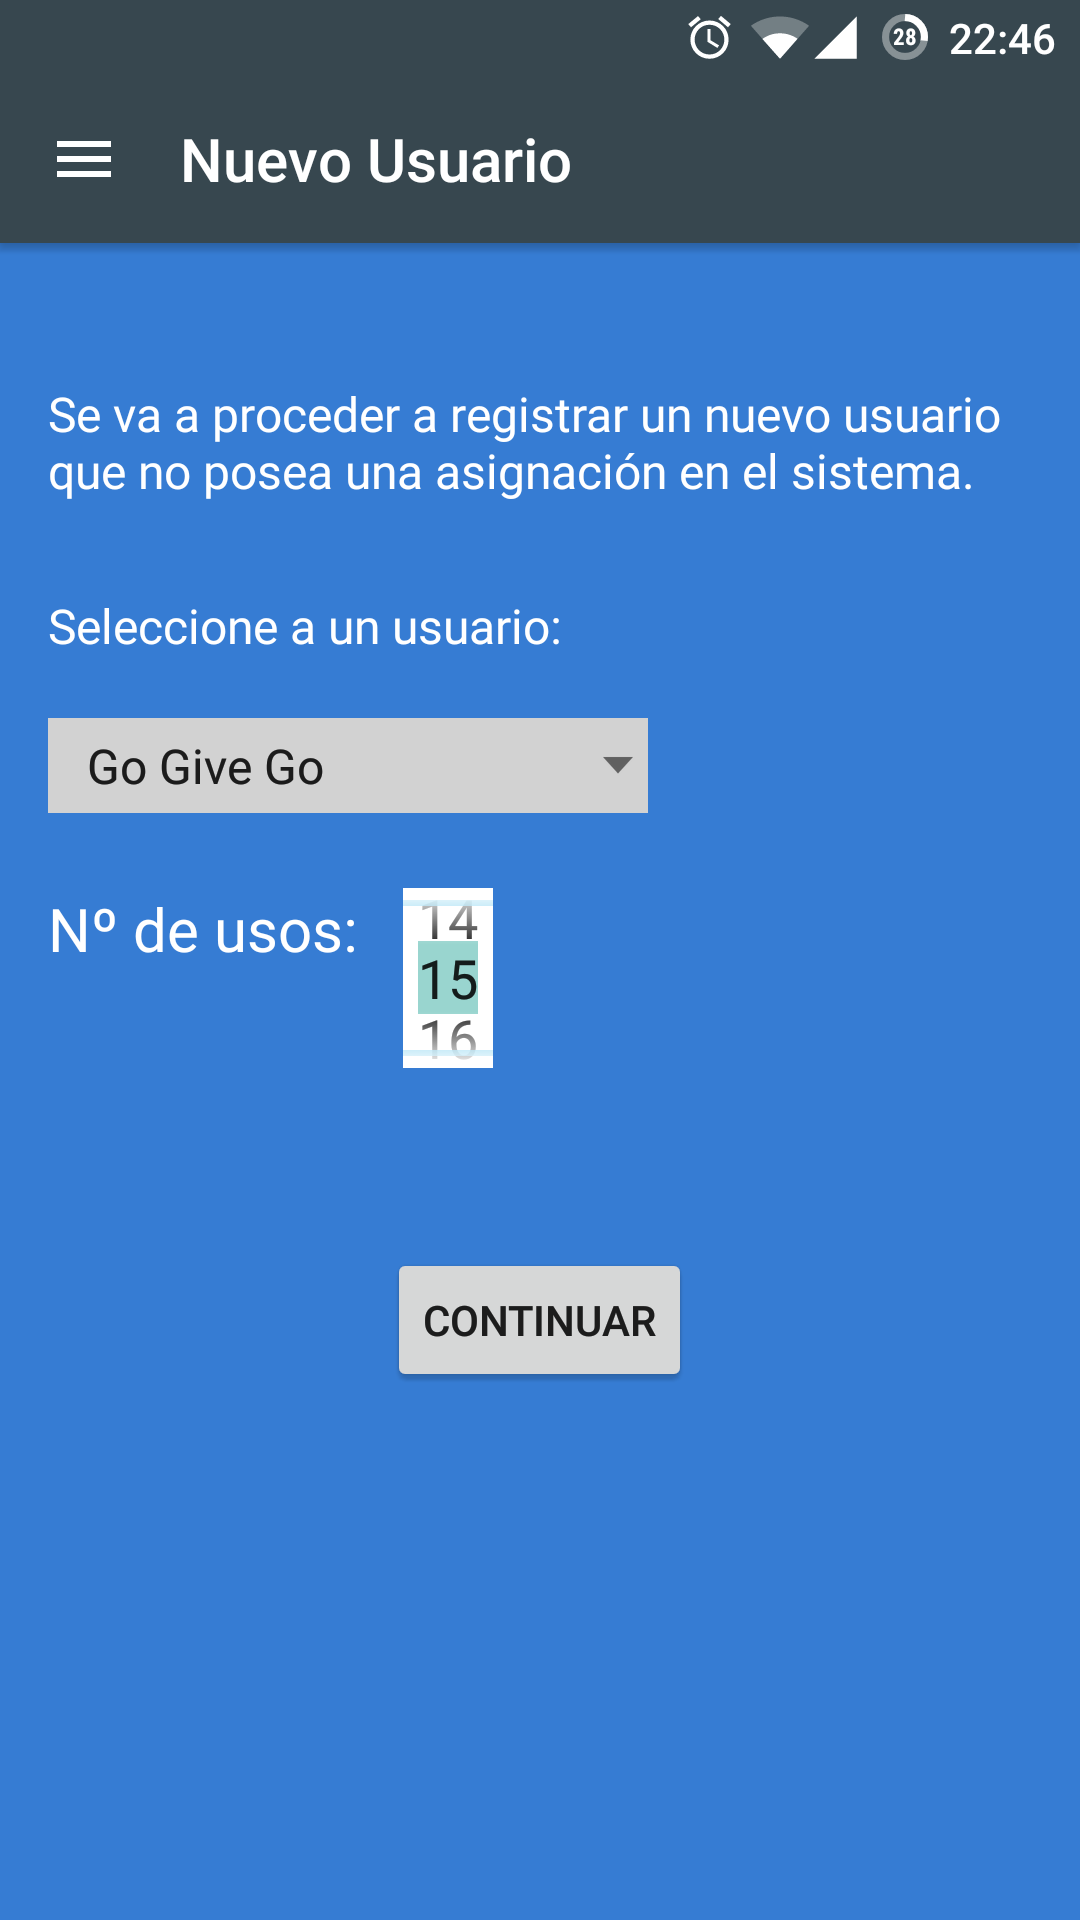
\includegraphics[width=0.3\textwidth]{./img/app/nuevoUsuario}
  \caption{Pantalla 'Nuevo usuario'.}
  \label{img:app:nuevoUsuario1}
\end{figure}  

\begin{figure}[H]
  \centering
  \subfloat{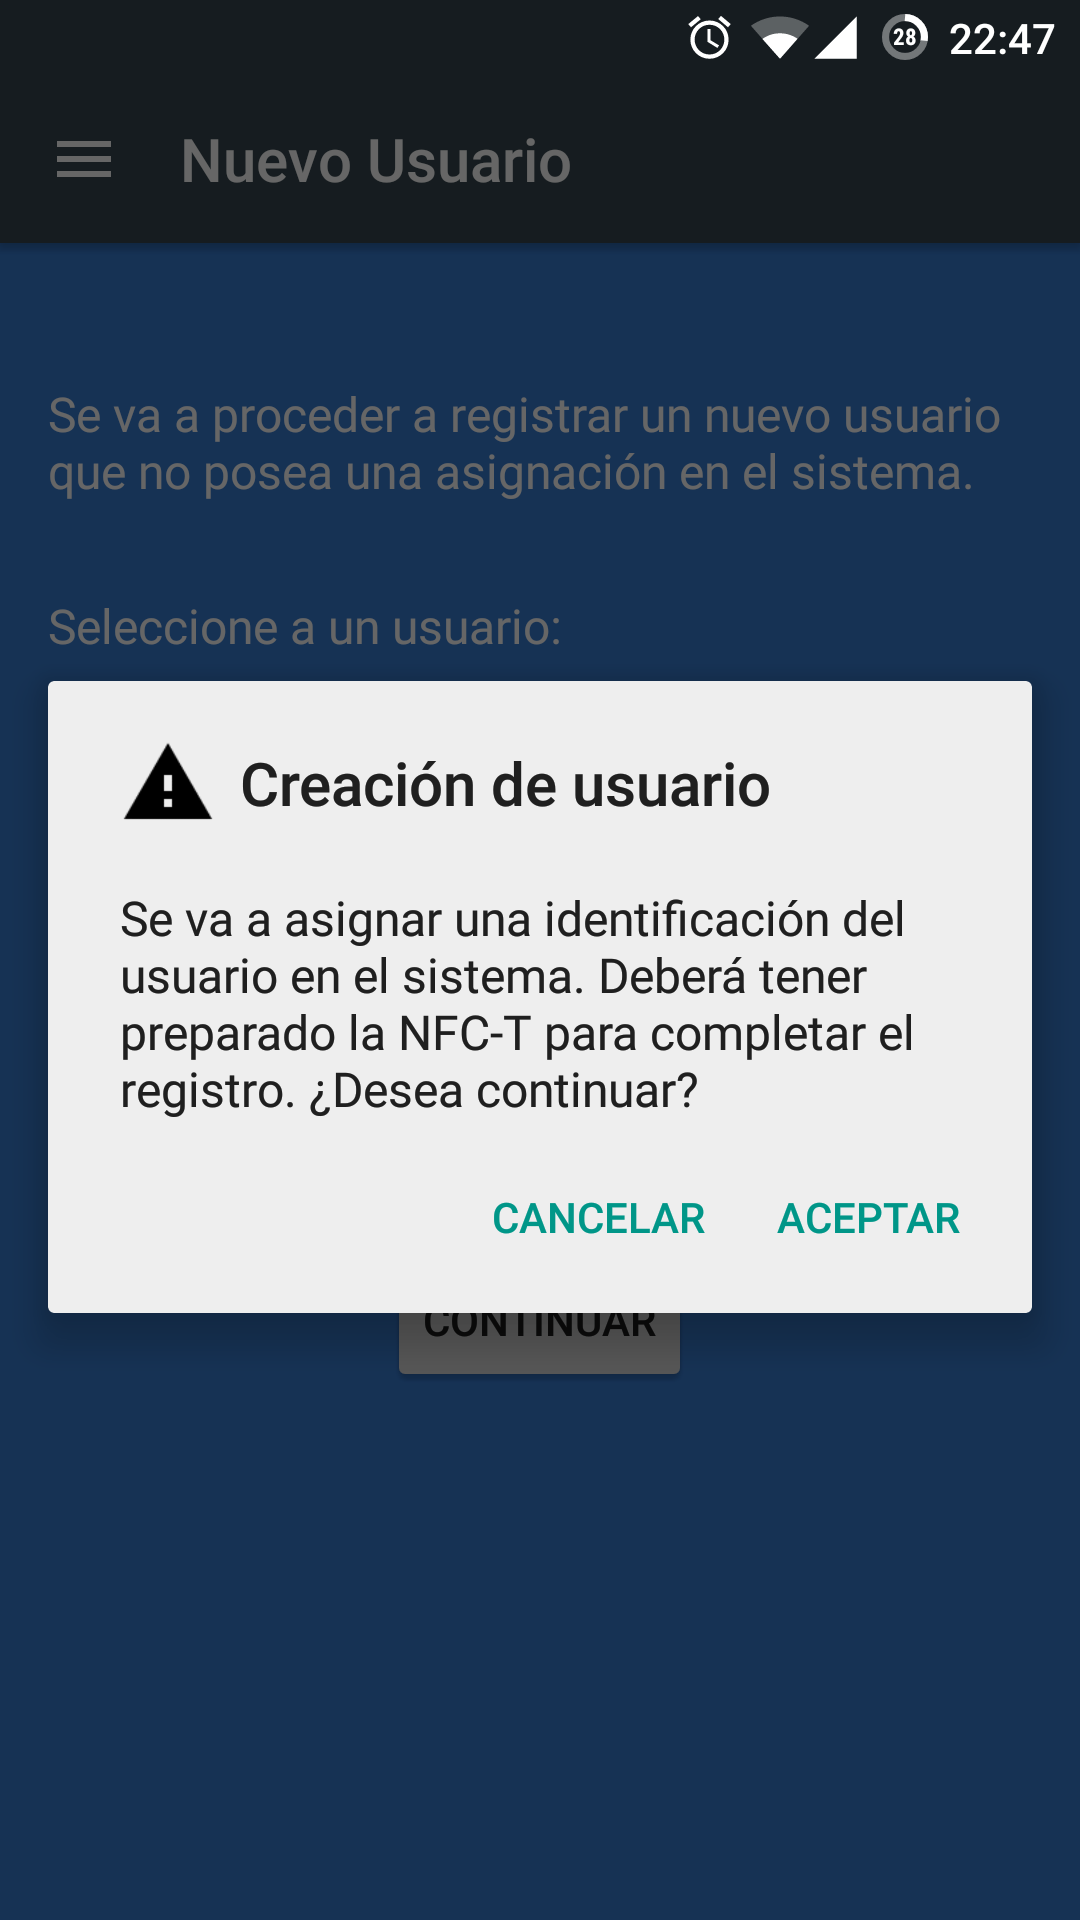
\includegraphics[width=0.35\textwidth]{./img/app/nuevoUsuarioDialog}}
  \null\hfill
  \subfloat{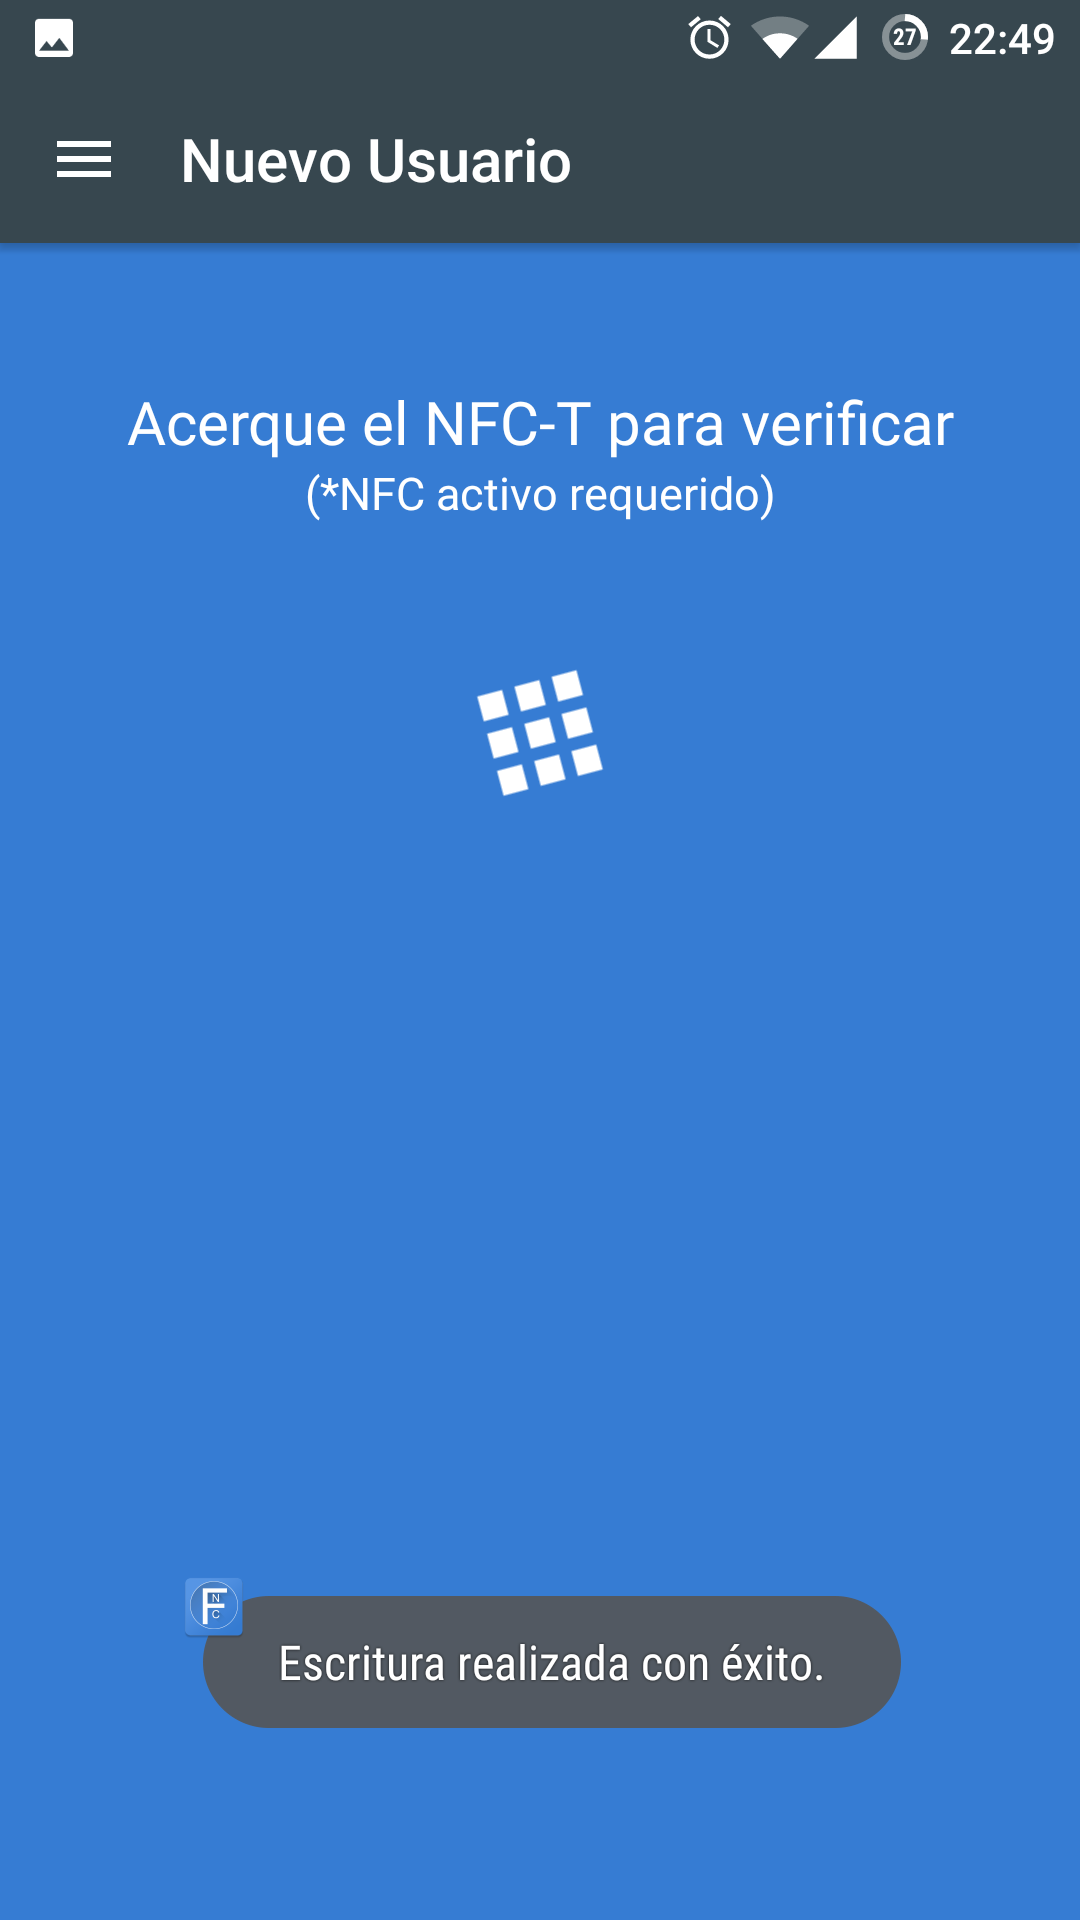
\includegraphics[width=0.35\textwidth]{./img/app/nuevoUsuarioAgregado}}
  \caption{Aviso de creación de un nuevo usuario y escritura de la tarjeta NFC.}
  \label{img:app:nuevoUsuario2}
\end{figure}

\subsection{Ver usuarios}
\label{App:AD:Ver usuarios}

Desde el menú se puede acceder a la pestaña de ver usuarios. Donde se muestra la información de la base de datos relativa  los usuarios del sistema actual. La figura \ref{img:app:verUsuarios} muestra la vista con varios usuarios y con un solo usuario en el sistema. Si no hubiera usuarios mostraría un mensaje avisando de que no hay usuarios disponibles.

\begin{figure}[H]
  \centering
  \subfloat{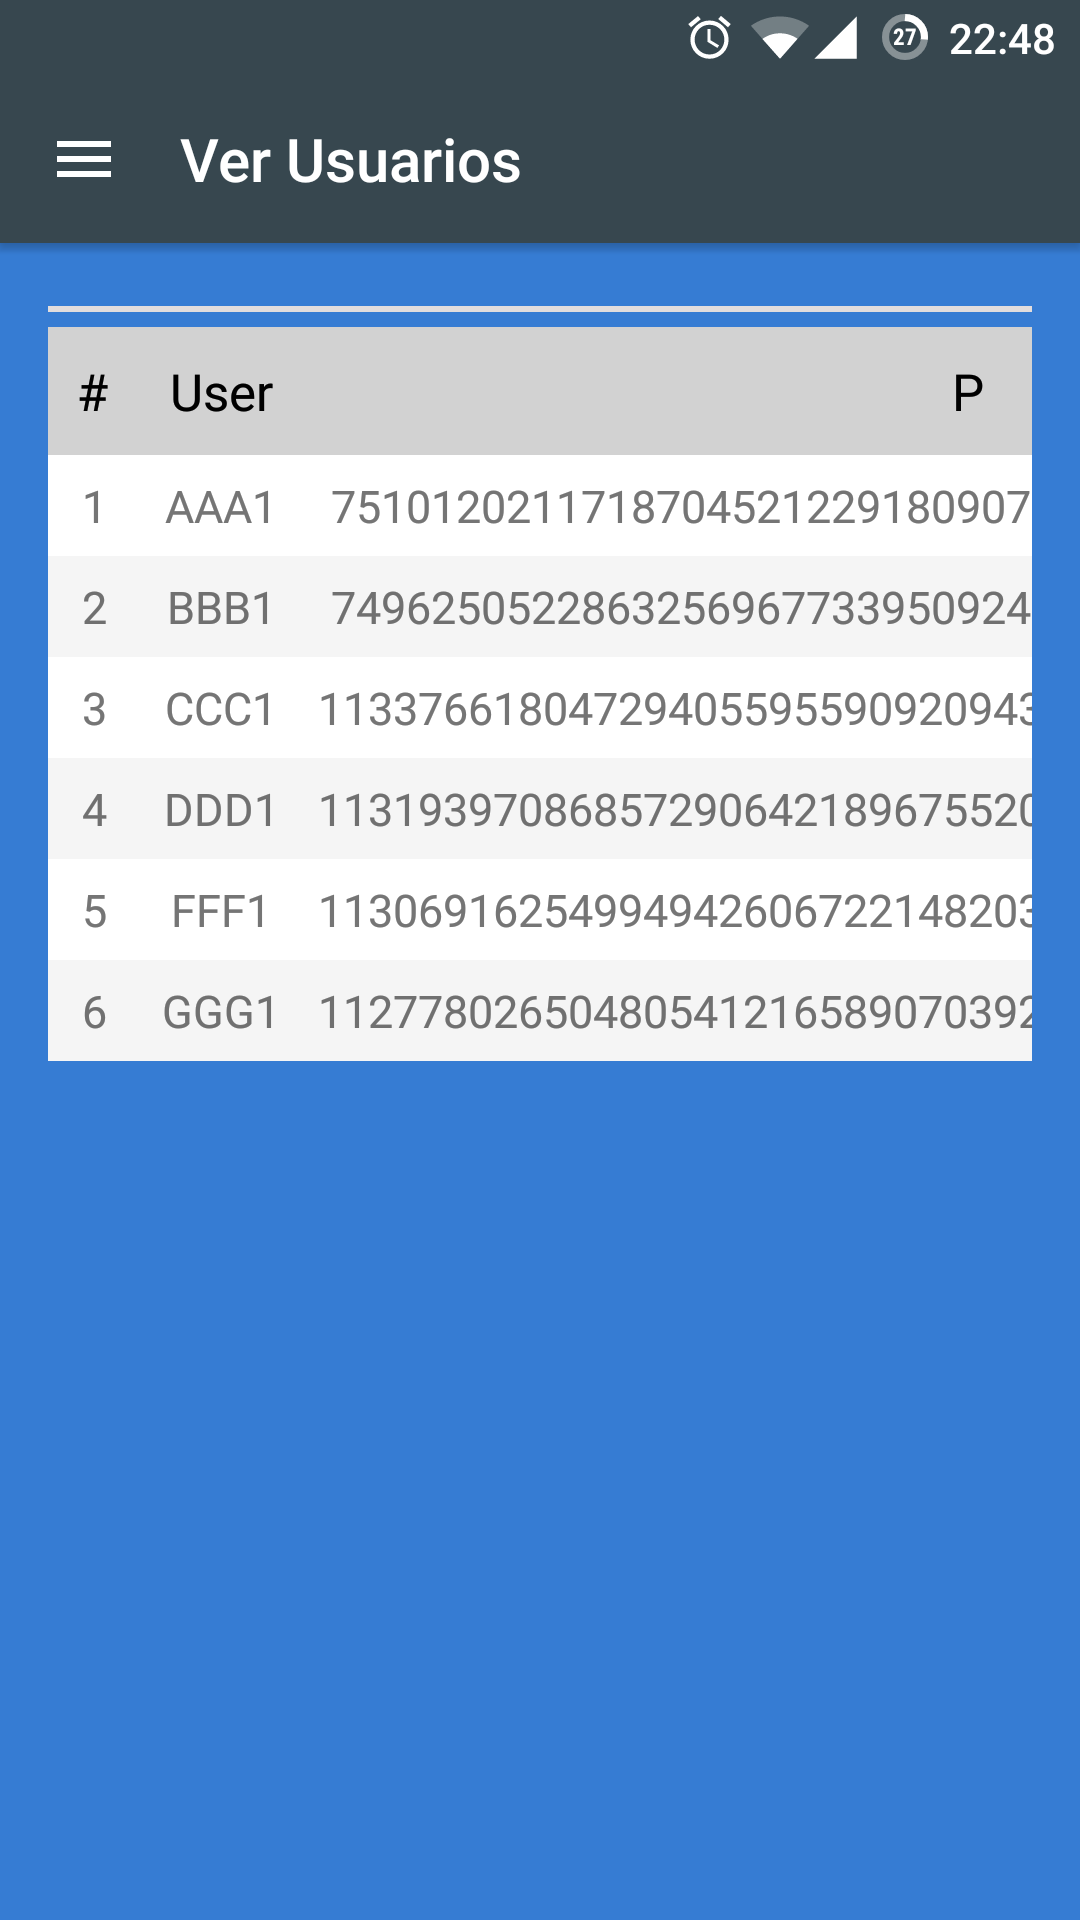
\includegraphics[width=0.35\textwidth]{./img/app/verUsuarios}}
  \null\hfill
  \subfloat{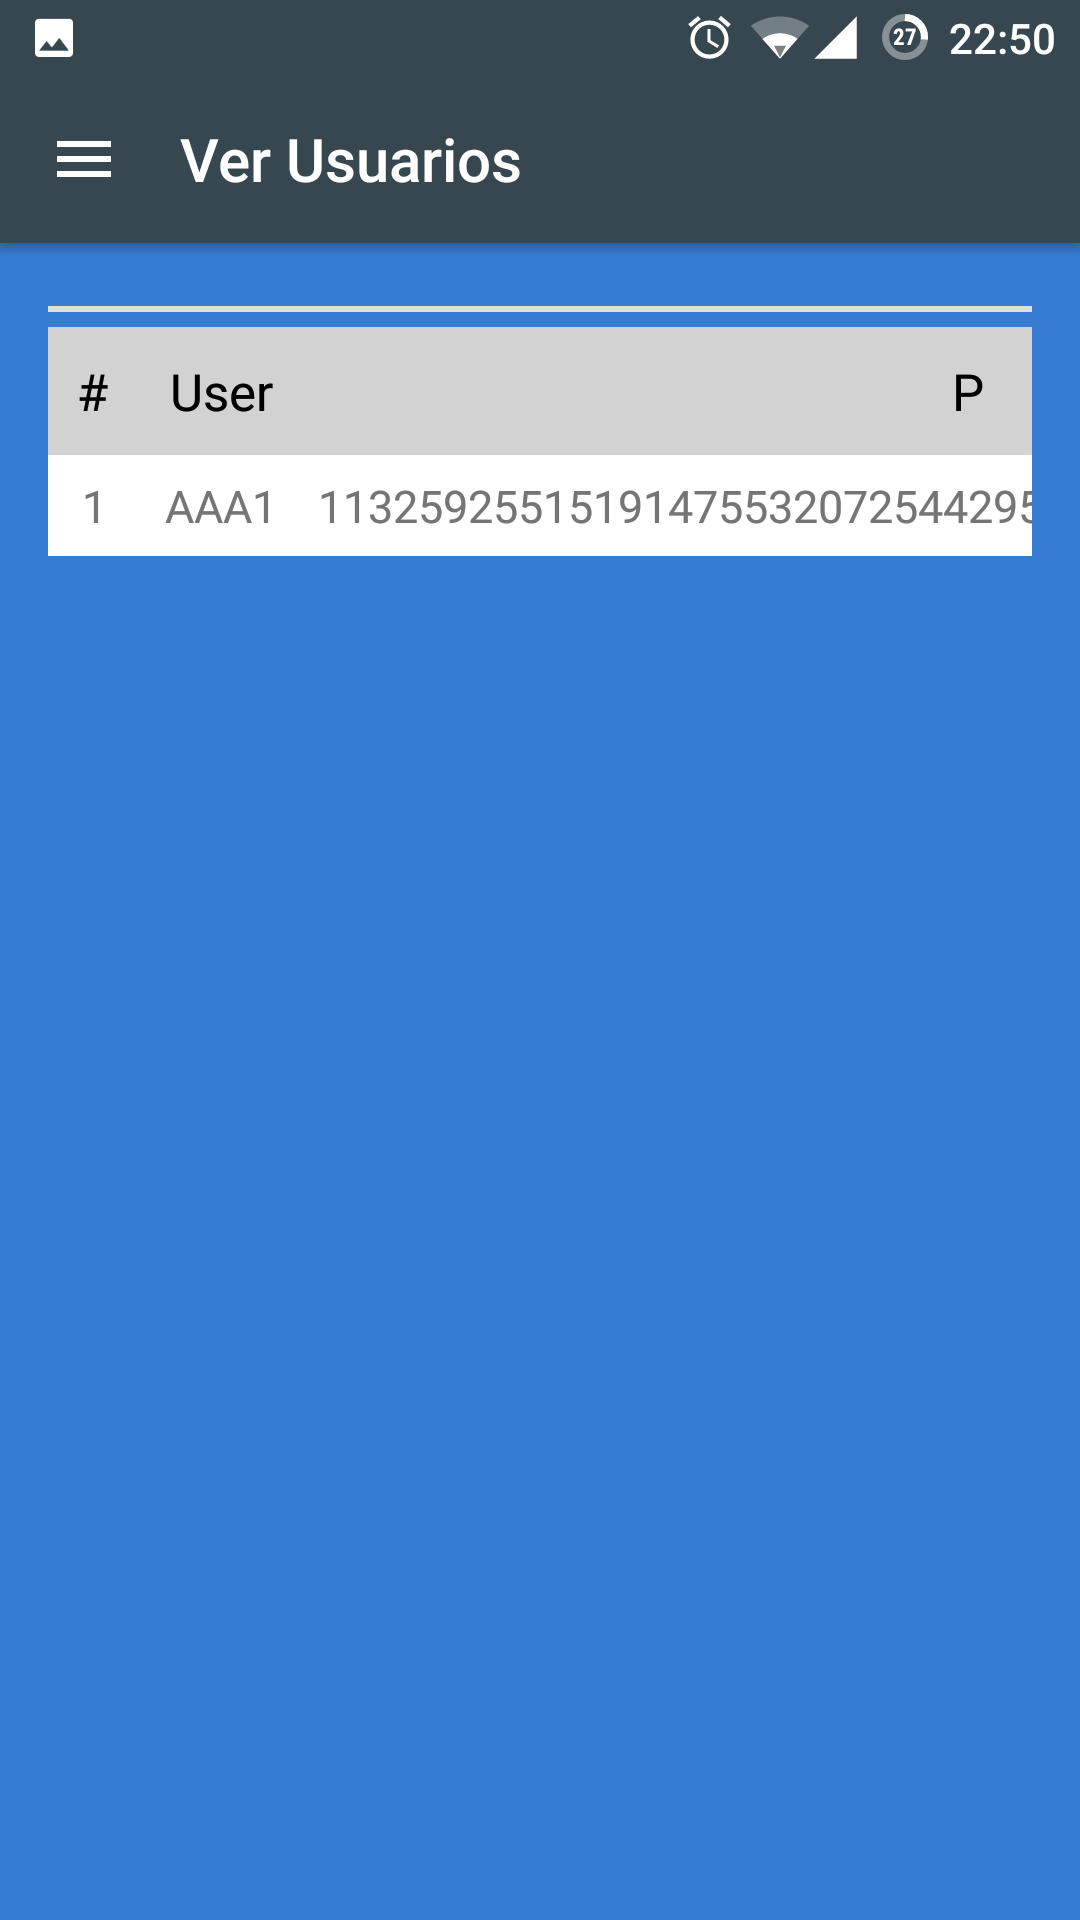
\includegraphics[width=0.35\textwidth]{./img/app/nuevoUsuarioInsertado}}
  \caption{Listado de varios usuarios y un usuario del sistema.}
  \label{img:app:verUsuarios}
\end{figure}

\subsection{Verificación}
\label{App:Verificacion}

Por último, el menú dispone la pestaña de verificación. En esta pestaña se avisa de que se puede aproximar una tarjeta NFC (con NFC activo en el dispositivo \textit{Android}) como indica la figura \ref{img:app:verificarNFC}.

\begin{figure}[H]
  \centering
  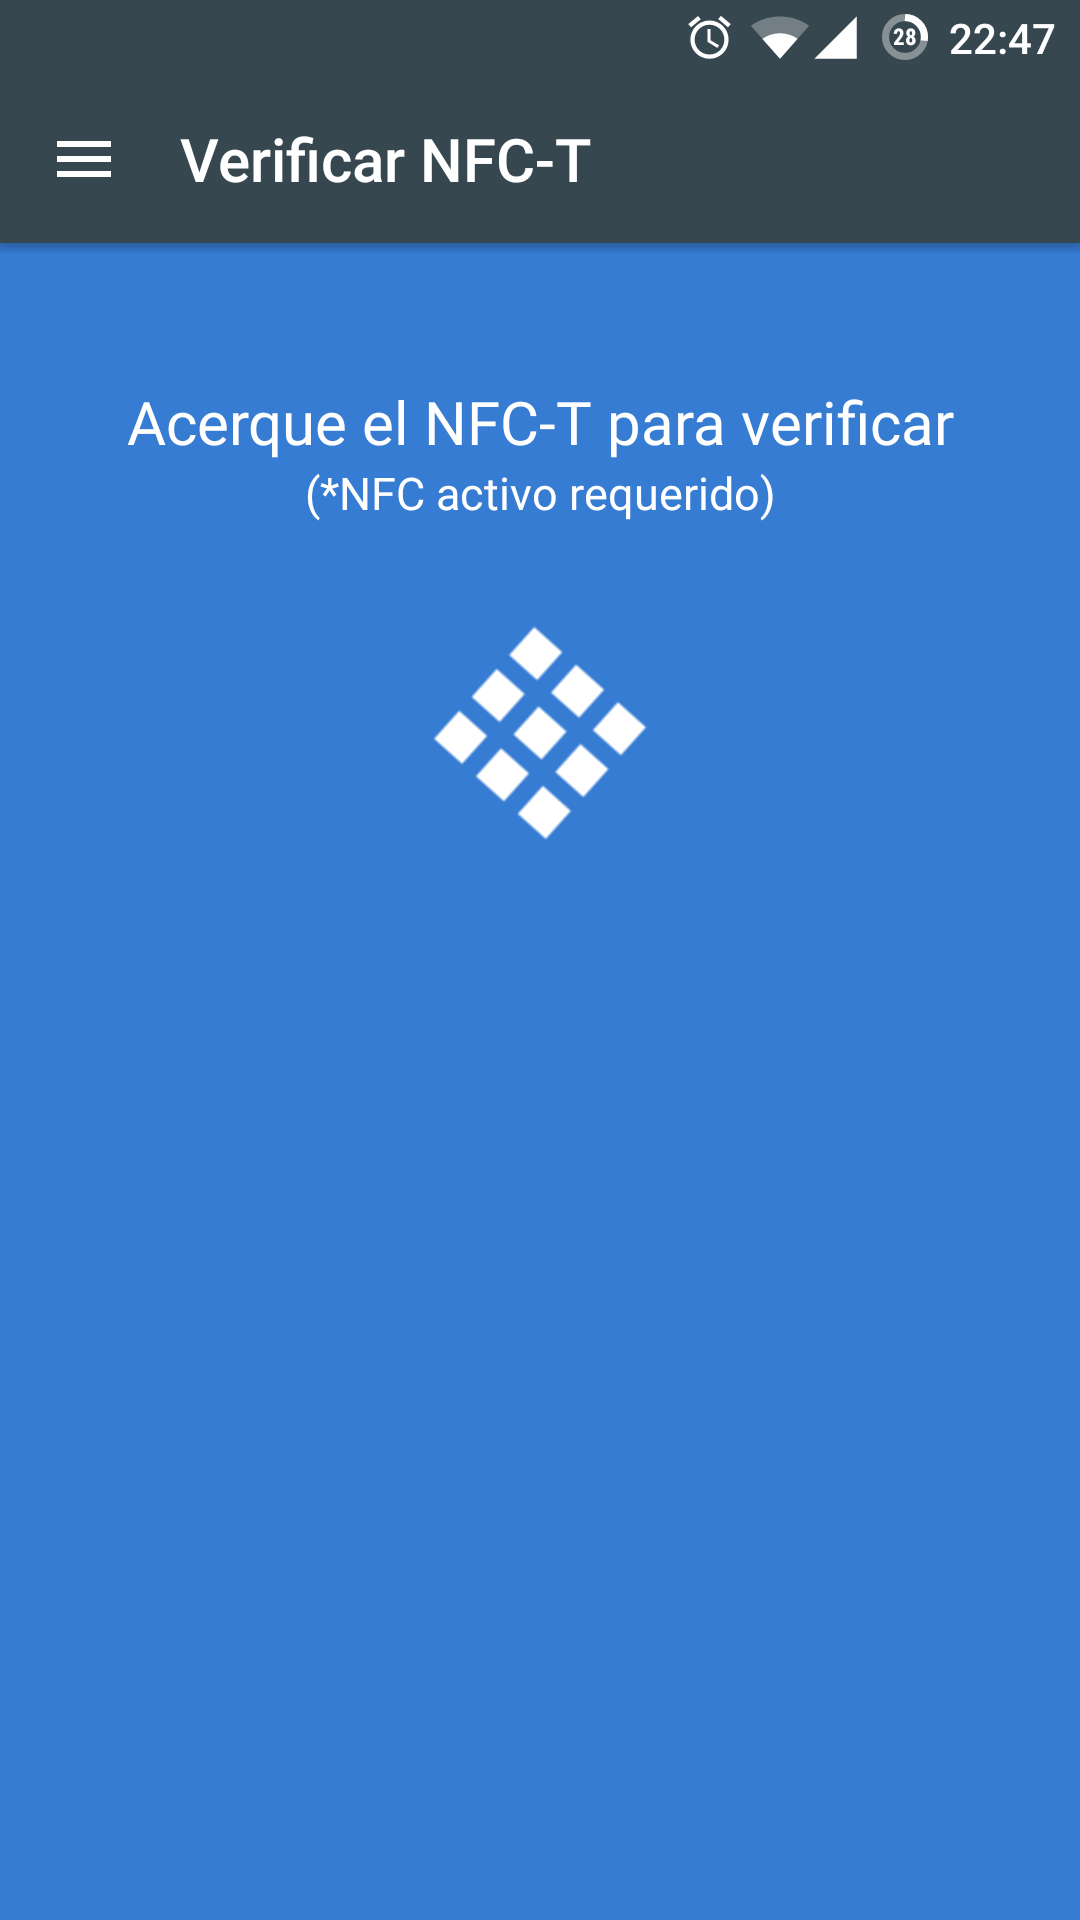
\includegraphics[width=0.3\textwidth]{./img/app/verificarNFC}
  \caption{Pantalla 'Verificar NFC'.}
  \label{img:app:verificarNFC}
\end{figure}  

Cuando el dispositivo detecta el contacto de una tarjeta NFC se lanzará automáticamente esta pantalla en la aplicación. Por lo que no es necesario encontrarse en esta pestaña cuando se acerque la tarjeta al dispositivo. Si el contenido es correcto se mostrará un mensaje de validación, sino mostrará un mensaje de error, ambos comportamientos se ven en la figura \ref{img:app:verificarNFC1}. Sin embargo, puede darse el caso de que no se escriba el nuevo contenido en la tarjeta tras verificarla. De esta forma, no se muestra el mensaje de escritura con éxito hasta que no se vuelva a acercar otra vez la tarjeta NFC, el comportamiento se observa en la figura \ref{img:app:verificarNFC2}.

\begin{figure}[H]
  \centering
  \subfloat{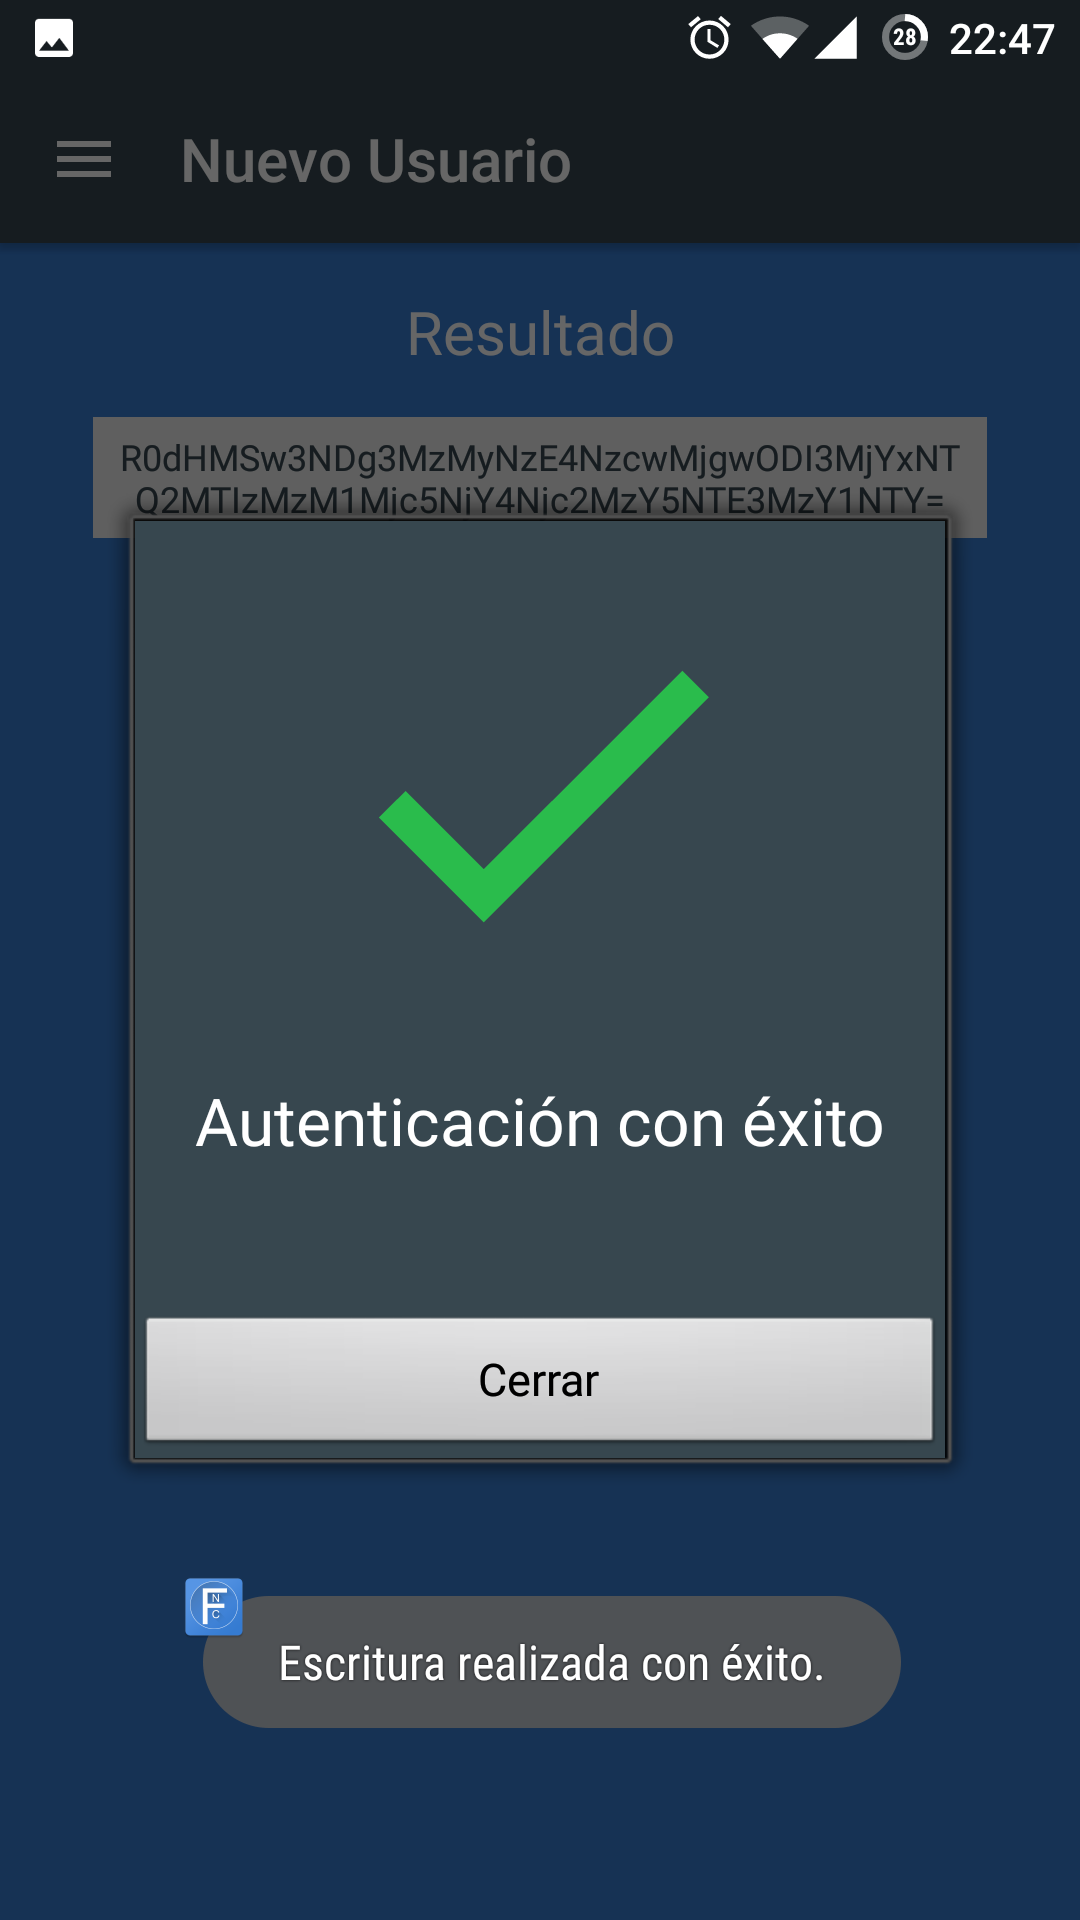
\includegraphics[width=0.35\textwidth]{./img/app/validacionExitoEscrito}}
  \null\hfill
  \subfloat{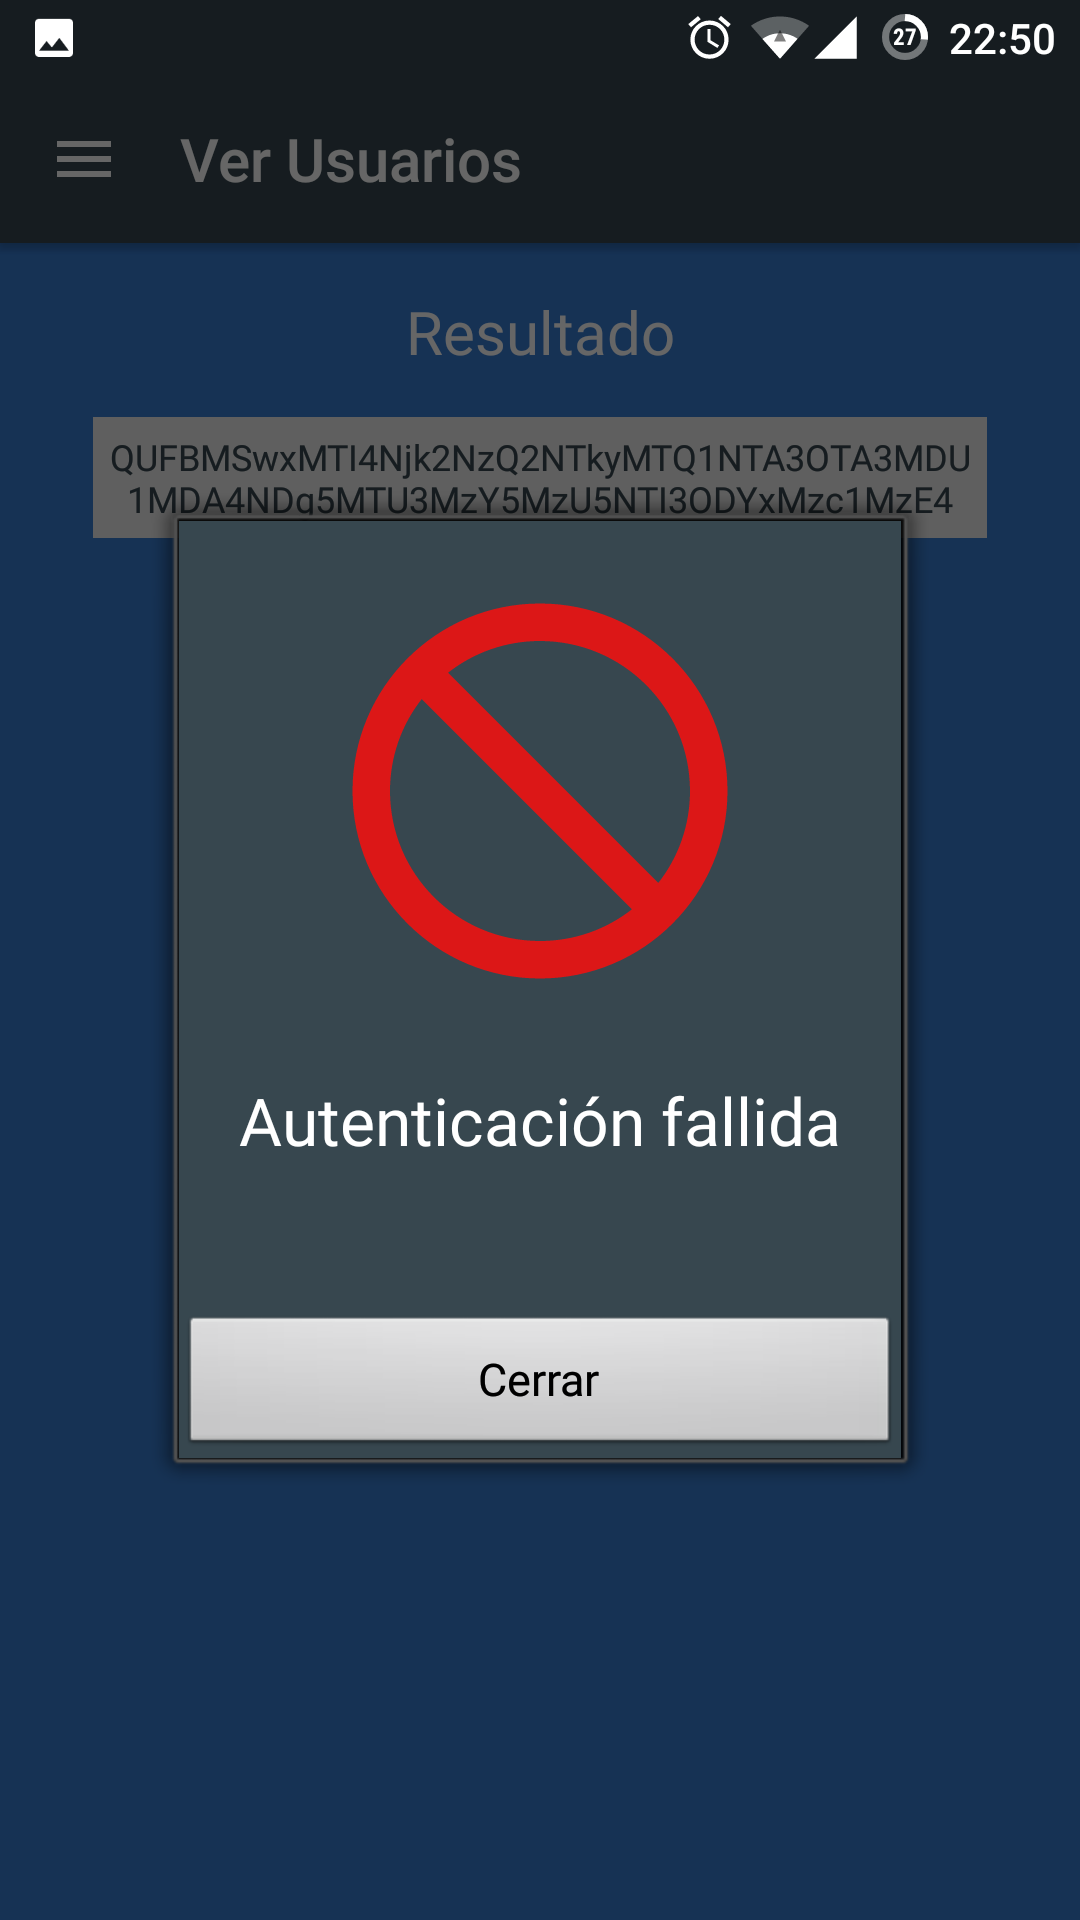
\includegraphics[width=0.35\textwidth]{./img/app/validacionFallida}}
  \caption{Verificar NFC válida común y fallida.}
  \label{img:app:verificarNFC1}
\end{figure}

\begin{figure}[H]
  \centering
  \subfloat{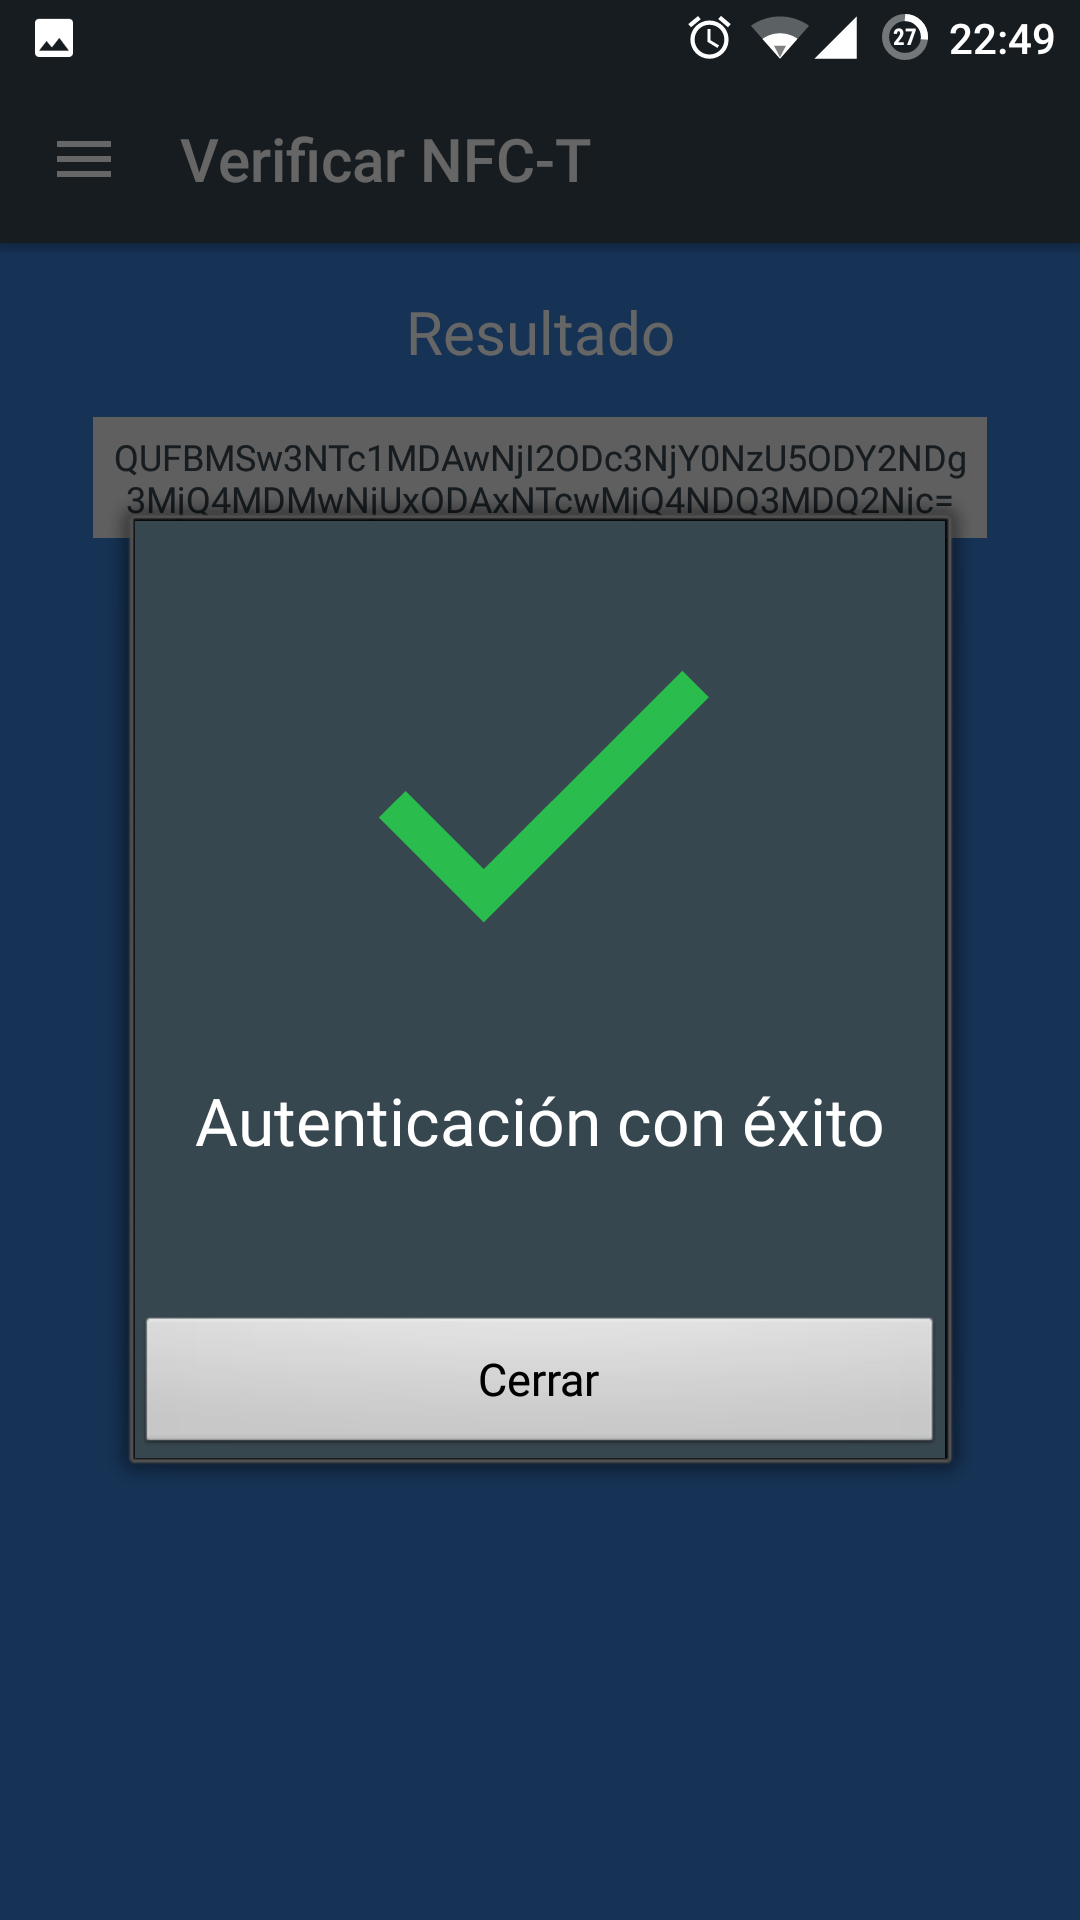
\includegraphics[width=0.35\textwidth]{./img/app/ValidacionExitoNoEscrito}}
  \null\hfill
  \subfloat{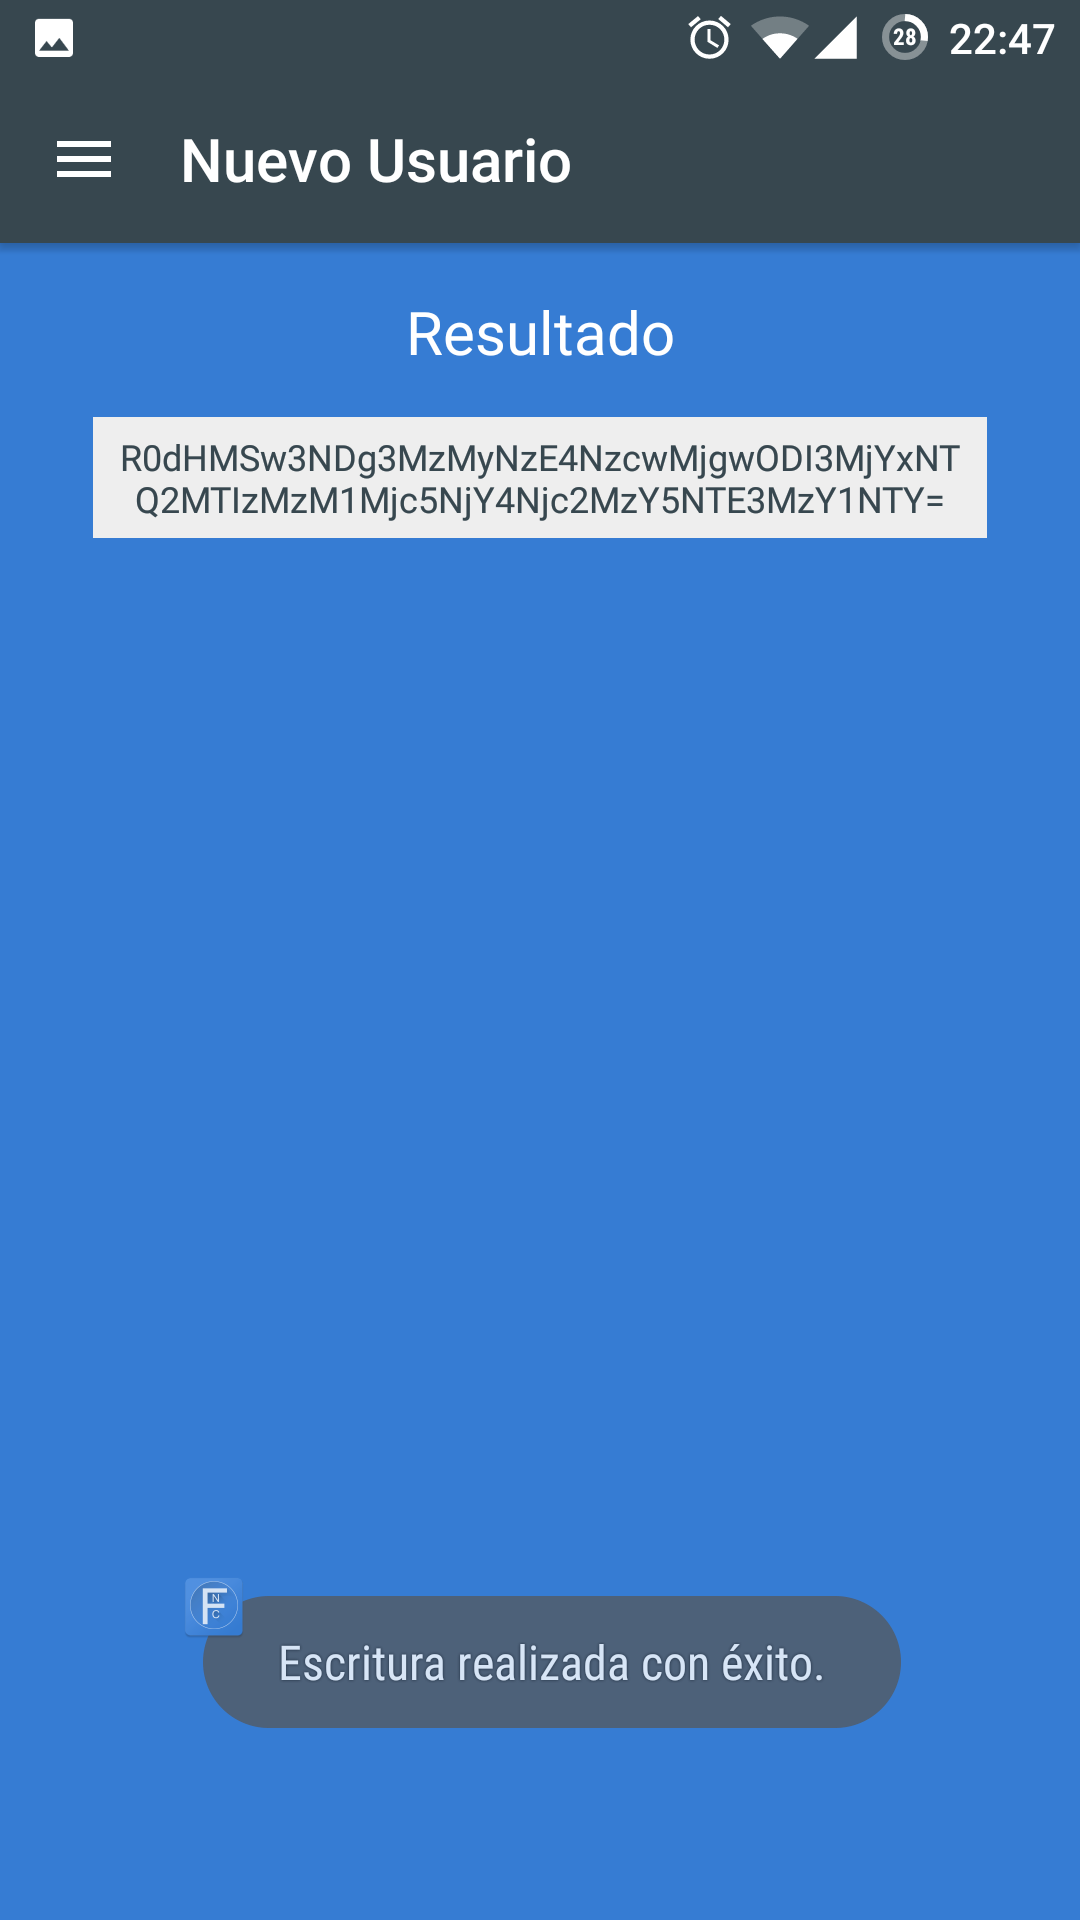
\includegraphics[width=0.35\textwidth]{./img/app/escrituraPostLectura}}
  \caption{Verificar NFC válida, con escritura realizada y sin ella.}
  \label{img:app:verificarNFC2}
\end{figure}

\section{Pruebas}
\label{App:Pruebas}

Para la comprobación y consecución de pruebas unitarias se ha elaborado un proyecto independiente para el testeo de la parte crítica de la aplicación. Ésta parte es la referida a la implementación de la seguridad y criptografía (\textit{véase apartado \ref{App:Seguridad y criptología}}).
\\\\
En cada uno de los métodos de la clase principal se ha testeado que su ejecución en distintos ámbitos y condiciones devuelve los resultados esperados cubriendo un alto porcentaje de código. Las pruebas se han centrado en el \textit{framework} de pruebas unitarias \textit{JUnit}\cite{junit} en su versión 4 elaborada para \textit{Eclipse}\cite{eclipse}.
\\\\
La descripción básica de la clase y su documentación es la recogida por la interfaz que implementa (la descripción en detalle de la clase de puede encontrar en el apartado \ref{App:Seguridad y criptología}). El resultado de los test JUnit se pueden observar en la figura \ref{img:junitTest} con una consecución de cobertura del código de más del 96\% realizado con el complemento \textit{EclEmma}\cite{eclemma} para este propósito. En la misma figura se muestra la prueba de consecución de cobertura código la clase objetivo. 

\begin{figure}[H]
  \centering
  \subfloat{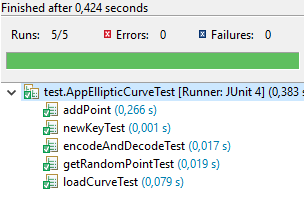
\includegraphics[width=0.45\textwidth]{./img/junitTest}}
  \null\hfill
  \subfloat{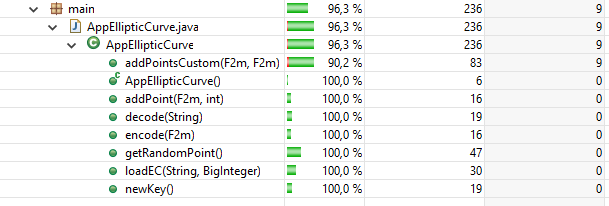
\includegraphics[width=0.5\textwidth]{./img/coveredCode}}
  \caption{Resultado del test JUnit y cobertura de código alcanzada durante el test JUnit.}
  \label{img:junitTest}
\end{figure}

En la realización de estas pruebas unitarias de la clase que implementa la interfaz \textit{AppEllipticCurveI}, clase principal que implementa la seguridad de la aplicación, se ha utilizado diferentes pruebas de ejecución del código utilizando \textit{Java Reflection}\cite{javaReflection} cuando se ha considerado oportuno. A modo de ejemplo se muestra en la figura el código del método principal \textit{loadEC} para la carga de una curva elíptica en el sistema.

\begin{figure}[H]
  \centering
  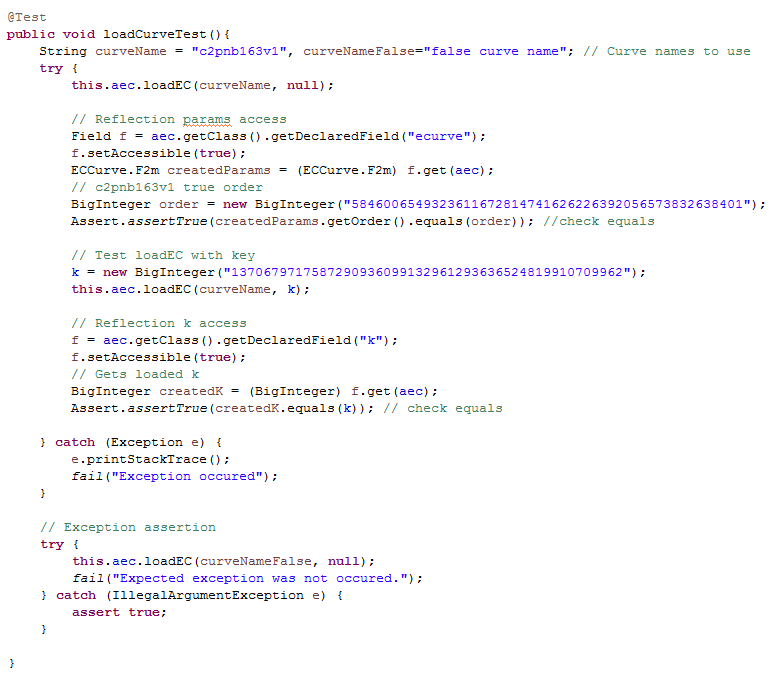
\includegraphics[width=0.75\textwidth]{./img/loadCurveTest}
  \caption{Script para el test de la creación de una curva elíptica.}
  \label{img:loadCurveTest}
\end{figure}

\end{document}
